%%%%%%%%%%%%%%%%%%%%%%%%%%%%%%%%%%%%%%%
%% Modelo TCC - PUC Minas
%% Arquivo Principal	
%%
%% Nome: Marciano Machado Saraiva
%% Data: 2021
%%%%%%%%%%%%%%%%%%%%%%%%%%%%%%%%%%%%%%%

\documentclass{abntpuc}
% \include{pacoteseclass}

% \let\cleardoublepage\clearpage


\usepackage{float}
\usepackage{hyperref}
\usepackage{graphicx}
\usepackage{adjustbox}
\usepackage{tabularx}
\usepackage{cite}
\usepackage{gensymb}
\usepackage{csquotes}
\usepackage{subfig}
\usepackage{listings}
\usepackage{footnote}
\usepackage[para,online,flushleft]{threeparttable}
\usepackage[table]{xcolor}

\definecolor{codegreen}{rgb}{0,0.6,0}
\definecolor{codegray}{rgb}{0.5,0.5,0.5}
\definecolor{codepurple}{rgb}{0.58,0,0.82}
\definecolor{backcolour}{rgb}{0.95,0.95,0.92}

\lstdefinestyle{mystyle}{
    backgroundcolor=\color{backcolour},   
    commentstyle=\color{codegreen},
    keywordstyle=\color{magenta},
    numberstyle=\tiny\color{codegray},
    stringstyle=\color{codepurple},
    basicstyle=\ttfamily\footnotesize,
    breakatwhitespace=false,         
    breaklines=true,                 
    captionpos=b,                    
    keepspaces=true,                 
    numbers=left,                    
    numbersep=5pt,                  
    showspaces=false,                
    showstringspaces=false,
    showtabs=false,                  
    tabsize=2
}

\lstset{style=mystyle}

\setlength{\cftbeforechapskip}{0pt}
\let\cleardoublepage\clearpage

\usepackage{etoolbox}
\makeatletter
\patchcmd{\scr@startchapter}{\if@openright\cleardoublepage\else\clearpage\fi}{}{}{}
\makeatother

\renewcommand\citeleft{(}
\renewcommand\citeright{)}


\setcitebrackets

\usepackage{blindtext}

\begin{document}

%%%%%%%%%%%%%%%%%%%%%%%%%%%%%%%%%%%%%%%
%% Modelo TCC - PUC Minas
%% 1 - Capa
%%
%% Nome:
%% Data:
%%%%%%%%%%%%%%%%%%%%%%%%%%%%%%%%%%%%%%%

% --- Campos que formarao: capa, folha de rosto, folha de aprovacao  ---

\curso{Inteligência Artificial e Aprendizado de Máquina}

\autor{Marciano Machado Saraiva}

\titulo{Mapeamento Intra-Anual do Uso e Cobertura da Terra Utilizando Inteligência Artificial e Sensoriamento Remoto} % Caixa alta

%\subtitulo{Subt{\'\i}tulo do Trabalho} % Caixa baixa

\cidade{Belo Horizonte}

\mes{Outubro}

\ano{2021}

\capa
\trabalho{Trabalho de Conclusão de Curso}

\grau{especialista}

\folharosto{}
% \listafiguras

% \listatabelas

% \listasiglas {
%   \sigla{S1}{Sigla 1}
%  \sigla{S2}{Sigla 2}
%   \sigla{S3}{Sigla 3}
% }

\newpage
\sumario{}
%%\include{3_FolhaDeAprovacao}
%%\include{4_DedicatoriaEAgradecimentos} %(elementos opcionais)
%%\include{4_Epigrafe} %(elemento opcional)
%\include{5_Resumo} 
%\include{6_ListaDeFigurasTabelasESumario} 


\chapter{Introdução}

Até a década de 70, a região do Oeste da Bahia permaneceu como um imenso território de reserva, parcialmente ocupado e com baixo nível de atividade econômica. A
partir dos anos 80, a região enfrentou uma rápida aceleração no ciclo de desenvolvimento, principalmente no que se refere as atividades que envolvem a agropecuária, como a criação de gado, produção de grãos e a fruticultura. Apenas na atividade agrícola, entre os anos de 1985 e 2020, a região teve uma expansão de mais de 10 vezes da área colhida, passando de aproximadamente 200 mil hectares em 1985 para cerca de 2,2 milhões de hectares em 2020, segundo os dados da pesquisa de Produção Agrícola Municipal (PAM) \cite{ibge2021pam}. Com esse acelerado crescimento das mudanças de uso e cobertura da terra, ter informações espacialmente explícitas sobre essas mudanças é fundamental para o planejamento e gestão sustentável dos recursos naturais, formulação de políticas públicas, gestão dos recursos hídricos, previsão da produção agrícola, entre outras aplicações sociais.

\renewcommand{\cleardoublepage}{}
\renewcommand{\clearpage}{}
\vspace{5mm}
\chapter{Contextualização}

Nos últimos anos, com o aumento na disponibilidade de imagens de satélite gratuitas, capacidade de processamento e eficientes técnicas de inteligência artificial, houve um forte crescimento na utilização de métodos automáticos para o mapeamento do uso e cobertura da terra. No Brasil, os dois projetos mais reconhecidos com esta finalidade são o TerraClass, do Instituto Nacional de Pesquisas Espaciais (INPE) \cite{coutinho2013uso} e o MapBiomas \cite{souza2020reconstructing}. O TerraClass produziu mapas anuais do uso e cobertura da terra para os biomas Amazônia e Cerrado em alguns anos, já o MapBiomas produz mapas anuais, para todo o território brasileiro, desde de 1985 até 2020, em sua última versão. Para mapeamentos anuais, os dois projetos cumprem muito bem o seu papel, de gerar informações anuais de qualidade sobre o uso e cobertura da terra. Porém, quando precisamos de informações intra-anuais, ou seja, identificar mudanças que ocorrem de um mês para o outro e até de uma semana para a outra, tanto o TerraClass quanto o MapBiomas não conseguem nos fornecer essas informações. Na agricultura, por exemplo, esses projetos conseguem nos dizer se uma determinada região foi cultivada ou não em um determinado ano, porém não conseguem nós dizer quantos ciclos de plantio/colheita essa região teve em um único ano-safra e nem quais culturas foram plantadas em cada ciclo, informação essencial para muitos tipos de aplicações, como a gestão de recursos hídricos e previsão da produção agrícola. 

\renewcommand{\cleardoublepage}{}
\renewcommand{\clearpage}{}
\vspace{5mm}
\chapter{Descrição do Problema e da Solução Proposta}

Diante desse contexto, este trabalho tem como objetivo desenvolver uma metodologia para permitir a geração de mapas do uso e cobertura da terra na mesorregião do Extremo Oeste Baiano, no estado da Bahia, com uma periodicidade de 16 dias. 

Para facilitar o entendimento do problema e da solução proposta, utilizamos a técnica dos 5W's, que consiste em responder as seguintes perguntas:

\textbf{Why?}: Identificar as variações intra-anuais do uso e cobertura da terra, como ciclos de plantio e colheita na agricultura, é fundamental para o planejamento e a gestão sustentável dos recursos naturais, formulação de políticas, gestão dos recursos hídricos, previsão da produção agrícola, entre outras aplicações sociais.

\textbf{Who?}: As imagens foram obtidas do satélite Landsat 8, disponibilizadas pelo Serviço Geológico dos Estados Unidos (USGS, pela sigla em inglês), e dos satélites Sentinel 2A e 2B, gerenciados pela Agência Espacial Europeia (ESA, pela sigla em inglês). Os polígonos anotados com as classes de uso e cobertura que foram utilizados para o treinamento e validação dos modelos foram obtidos do LEM Dataset (\citeonline{sanches2018lem}, \citeonline{oldoni2020lem}). 

\textbf{What?}: Desenvolver uma metodologia que permita a geração de mapas do uso e cobertura da terra com uma periodicidade de 16 dias.

\textbf{Where?}: Mesorregião do Extremo Oeste Bahiano, no estado da Bahia.  

\textbf{When?}: Os dados anotados do LEM Dataset foram obtidos nos períodos de Junho de 2017 à Maio de 2018, e de Outubro de 2019 à Setembro de 2020. Consequentemente, utilizamos esses mesmos períodos para obter as imagens de satélite e realizar o treinamento e validação dos modelos.  


\renewcommand{\cleardoublepage}{}
\renewcommand{\clearpage}{}
\vspace{5mm}
\chapter{Coleta de Dados}

Nas próximas seções, apresentaremos quais dados utilizamos neste trabalho para treinar e validar os modelos e como eles foram coletados. 
  
% \section{Área de Estudo}

% A mesorregião do Extremo Oeste da Baiano, na Bahia, é composta por 24 municípios que representam, juntos, uma área de aproximadamente 11,7 Mha (Figura \ref{fig:area_de_estudo}). A área destinada à atividade agrícola, entre os anos de 1985 e 2020, teve uma expansão de mais de 10 vezes, passando de 201.155 ha em 1985 para 2.275.160 ha em 2020, segundo os dados da pesquisa de Produção Agrícola Municipal (PAM), do Instituto
% Brasileiro de Geografia e Estatística (IBGE) \cite{ibge2021pam}. Os principais produtos cultivados são: soja, milho, algodão, e feijão, além de alguns cultivos frutíferos.

% \begin{figure}[H]
% \centering
% \caption{Representação da mesorregião do Extremo Oeste da Bahia, área de estudo utilizada como o foco deste trabalho.}
% \label{fig:area_de_estudo}
% 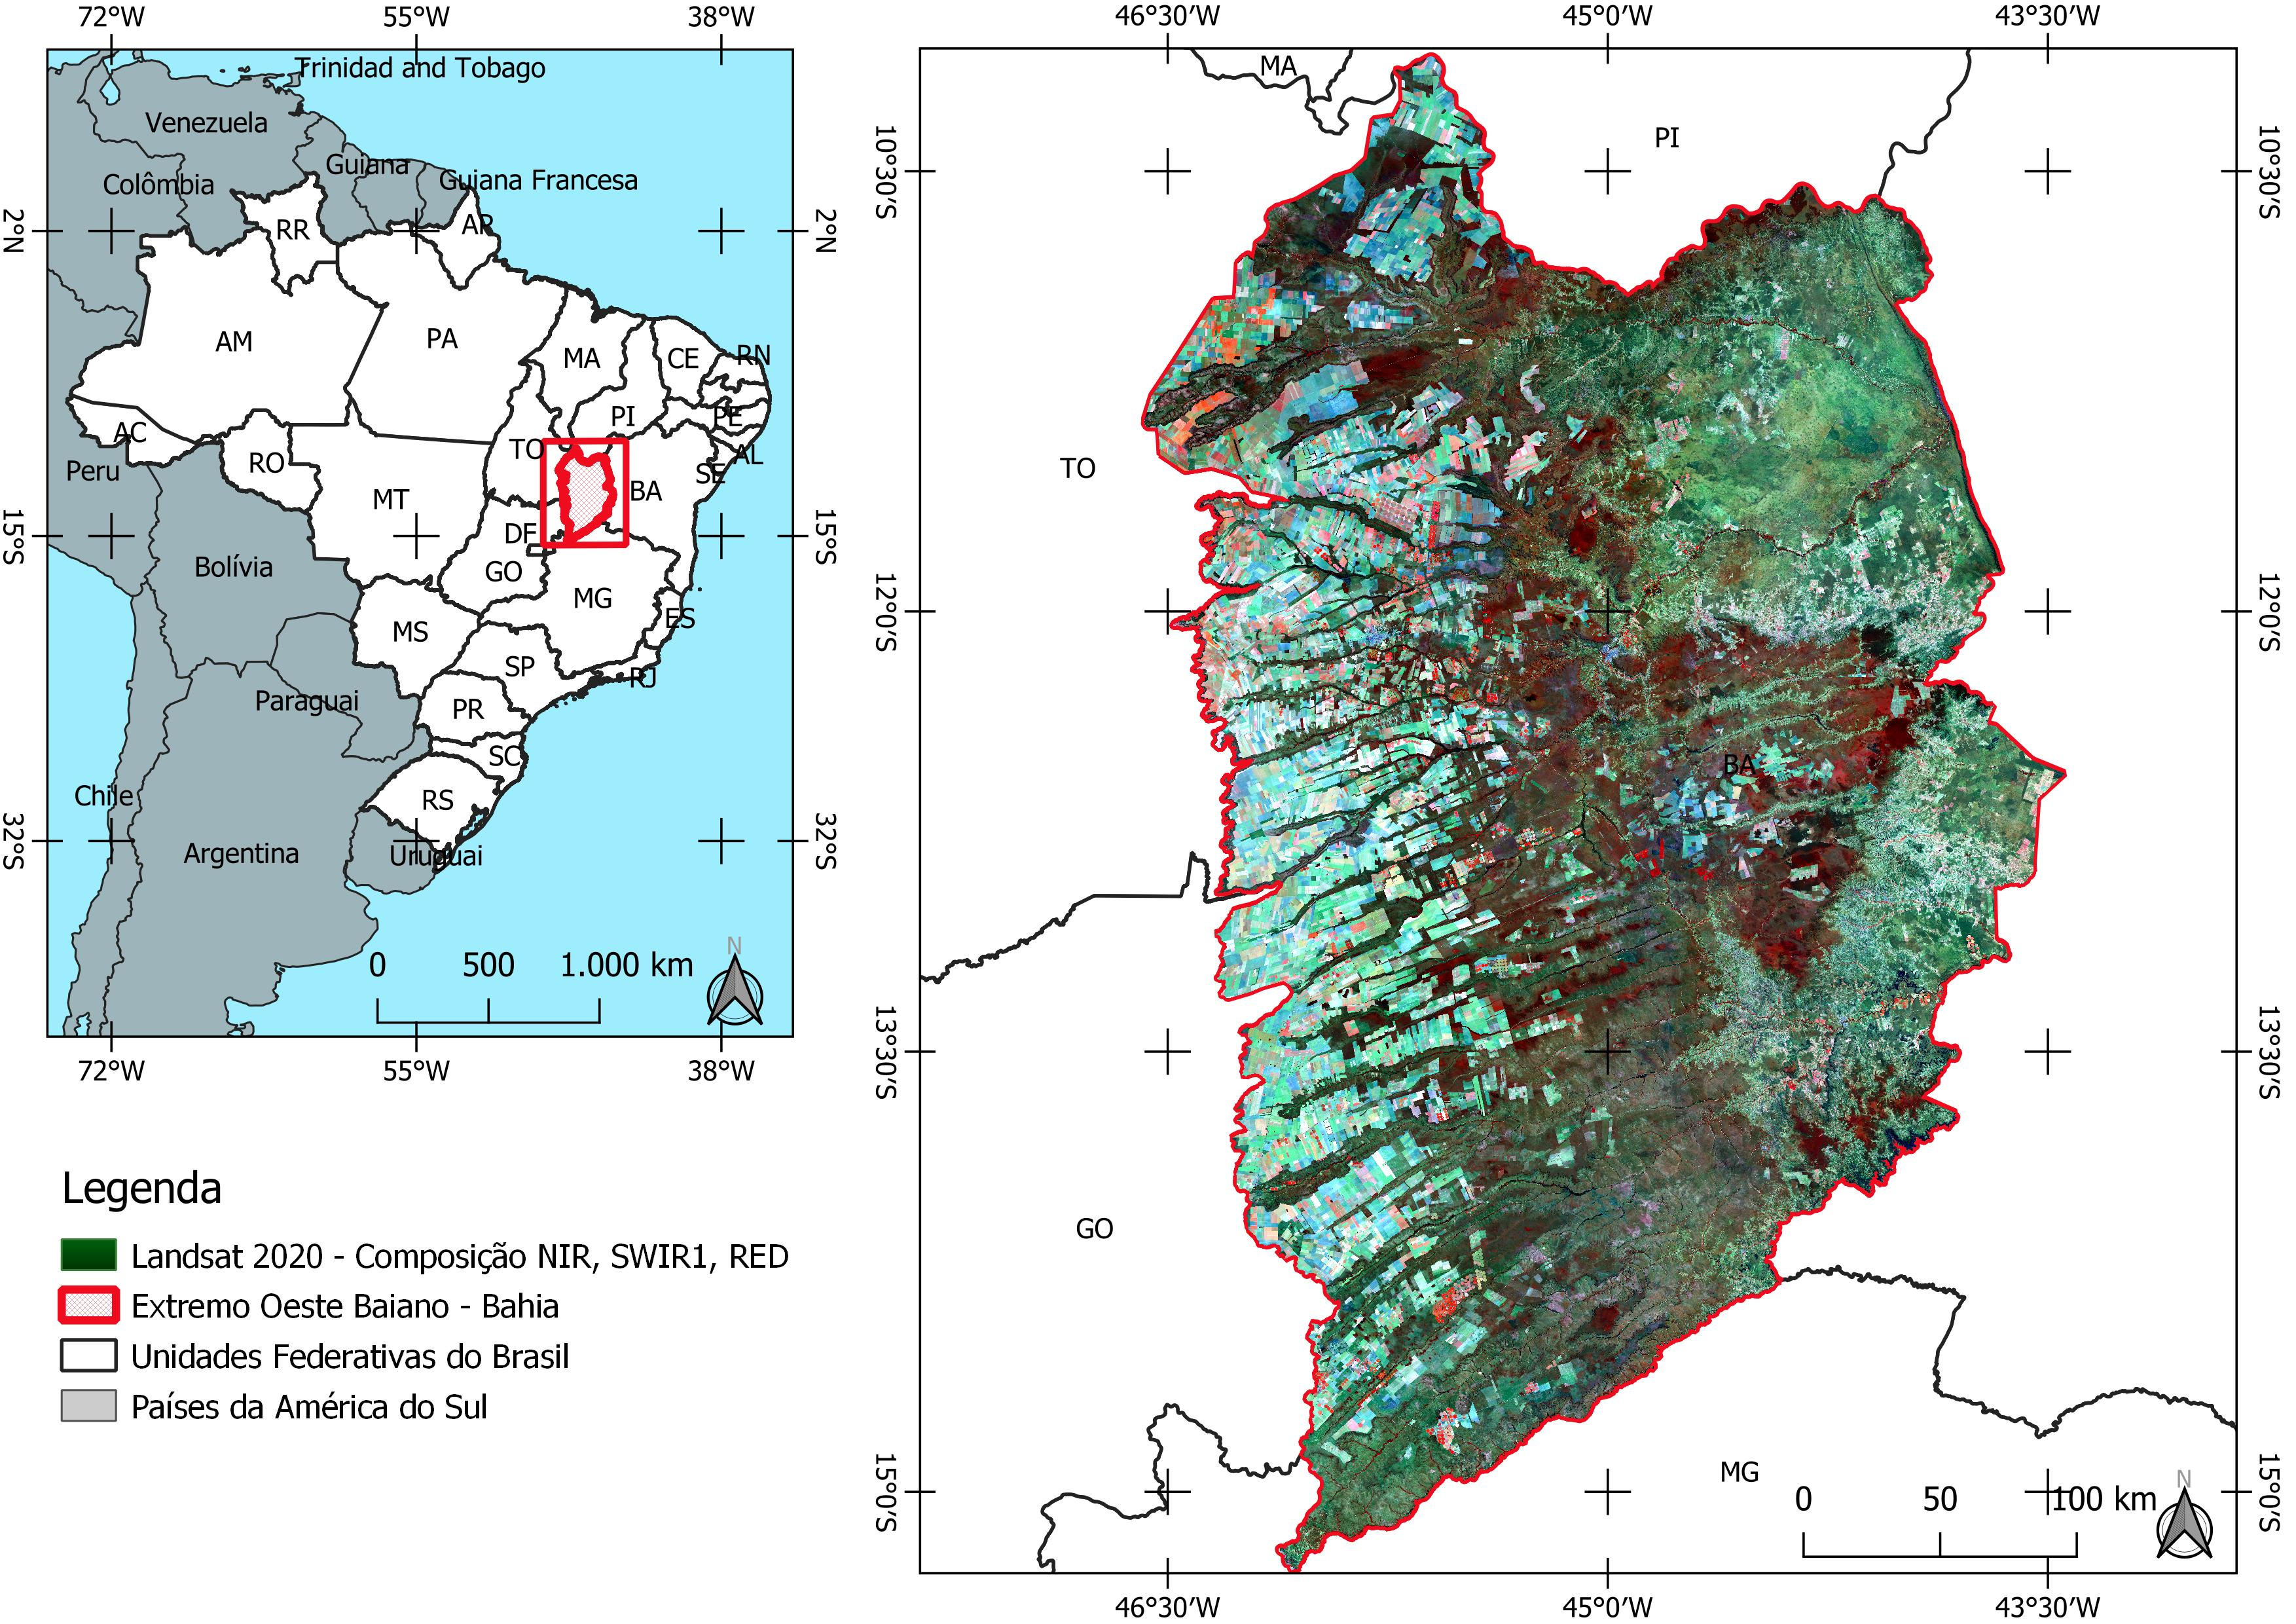
\includegraphics[width=0.6\textwidth]{figuras/area_de_interesse.jpg}
% \end{figure}

\section{Dados de Referência}

Um dos grandes desafios no mapeamento do uso e cobertura da terra é encontrar dados de referência de qualidade com o conjunto de características que se deseja estudar. Neste trabalho, utilizamos dois conjuntos de dados produzidos pelo Instituto Nacional de Pesquisas Espaciais (INPE) em parceria com a Pontifícia Universidade Católica do Rio de Janeiro (PUC Rio), o LEM Dataset e seu sucessor chamado LEM+ Dataset (Tabela \ref{tab:conjunto_de_dados}). O LEM Dataset foi construído após dois trabalho de campo realizados no município de Luís Eduardo Magalhães (LEM), na Bahia, entre junho de 2017 e março de 2018, período correspondente a segunda (estação seca) e a primeira (estação chuvosa) safra brasileira, respectivamente. já o LEM+ Dataset reúne dados coletados de outubro de 2019 a setembro de 2020 (um ano agrícola brasileiro) de Luís Eduardo Magalhães e outros municípios no oeste do estado da Bahia.    

\begin{table}[H]
\caption{Dados contendo os polígonos e as classes que foram utilizados como referência (\textit{Ground truth}) para este trabalho.}
\label{tab:conjunto_de_dados}
\begin{adjustbox}{width=\textwidth}
\begin{tabular}{|l|l|l|l|l|}
\hline
Conjunto de dados & Início     & Fim        & Área Mapeada & Referência \\ \hline
LEM Dataset       & 01/06/2017 & 31/05/2018 & 56.983 ha    & \cite{sanches2018lem} \\ \hline
LEM+ Dataset      & 01/10/2019 & 30/09/2020 & 251.038 ha   & \cite{oldoni2020lem}  \\ \hline
\end{tabular}
\end{adjustbox}
\begin{tablenotes}
\item[1] Os dados do LEM Dataset foram baixados em \url{http://www.dpi.inpe.br/agricultural-database/lem/dados/shp/classes_mensal_LEM_buffer_cut_v2.zip}, acesso em 01/08/2021. \\
\item[2] Os dados do LEM+ Dataset foram baixados em \url{https://md-datasets-public-files-prod.s3.eu-west-1.amazonaws.com/e0bd4285-03b8-494b-bc4d-fc89d80e6bd0}, acesso em 01/08/2021.
\end{tablenotes}
\end{table}

Com base em informações coletadas em campo, sensoriamento remoto óptico de imagens de séries temporais (Sentinel 2A e 2B / MSI e Landsat-8 / OLI) e perfis de NDVI (MODIS/Terra), os analistas conseguiram produzir esses dois conjuntos de dados que possibilitaram acompanhar, mensalmente, as mudanças de uso e cobertura da terra para os ano-safra em que ocorreram esses trabalhos de campo. A Figura \ref{fig:serie_imagens_exemplo_lemdataset} apresenta um exemplo de como estão organizados os dados de referência.  

\begin{figure}[H]
    \centering
    \caption{Exemplo de uma série temporal imagens de satélite em composição falsa cor (NIR, SWIR1, red) (a) e o índice de vegetação NDVI MODIS (b) usado para mapear, mensalmente, a classe de uso da terra  para as coordenadas -45,739369 e -12,156452 (lon, lat) no período de 01/10/2019 à 30/09/2020.}
    \label{fig:serie_imagens_exemplo_lemdataset}
    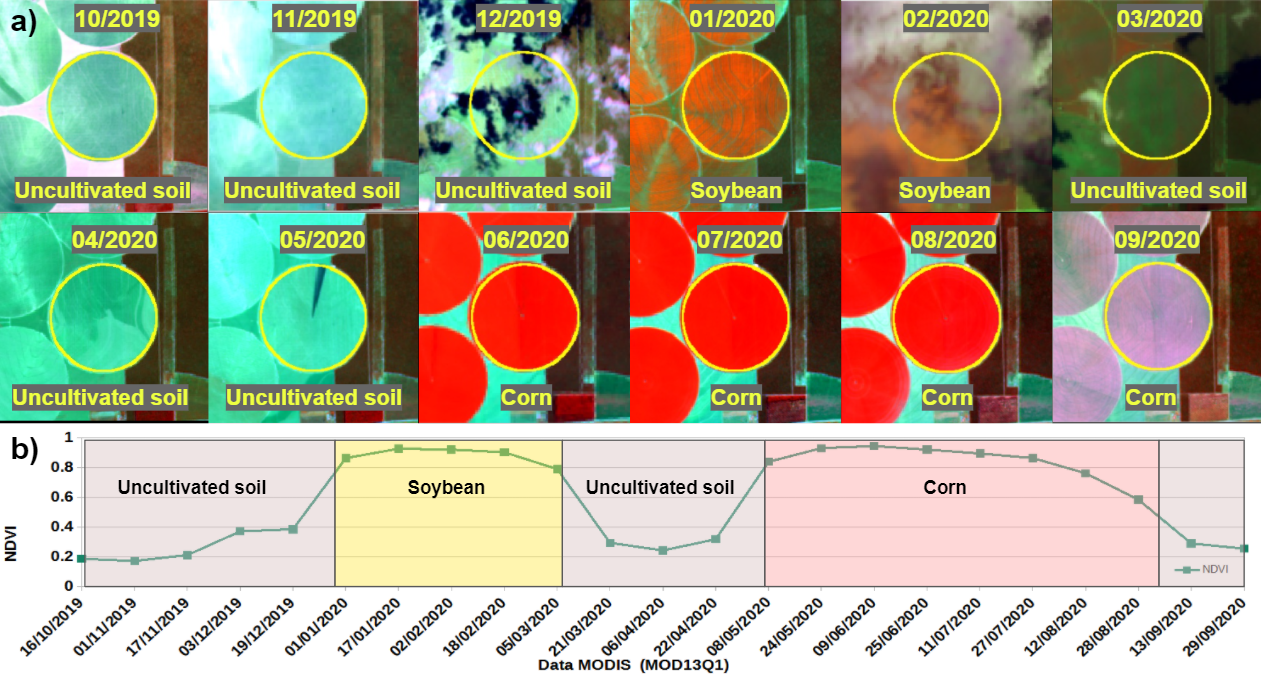
\includegraphics[width=0.7\textwidth]{figuras/exemplo_serie_temporal.png}
\end{figure}


\section{Imagens de satélite}

As imagens que utilizamos neste trabalho foram obtidas dos satélites Landsat 8 (sensor OLI), que possui como provedor oficial das imagens o serviço geológico dos Estados Unidos (USGS), e os satélites Sentinel 2A e 2B (sensor MSI) que são administrados pela Agência Espacial Europeia (ESA). 

A USGS disponibiliza as imagens do satélite Landsat 8 em duas diferentes coleções de imagens, a \textit{Collection 1} e a \textit{Collection 2} \cite{eros2017landsat}. As imagens disponíveis da \textit{Collection 2} possuem um maior nível de qualidade e correções. Por este motivo, neste trabalho utilizamos apenas as imagens disponíveis na \textit{Collection 2}. As imagens disponíveis na \textit{Collection 2} são agrupadas em dois diferentes níveis de qualidade, \textit{Tier 1} e \textit{Tier 2}  \cite{eros2017landsat}. As imagens disponíveis no \textit{Tier 1} são imagens com maior qualidade e Erro Quadrático Médio (RMSE) de registro menor ou igual a 12 metros \cite{eros2017landsat}, já as imagens disponíveis no \textit{Tier 2} possuem RMSE de registro maior que 12 metros. Neste trabalho, processamos apenas as imagens disponíveis no \textit{Tier 1} da \textit{Collection 2}.

A ESA disponibiliza as imagens dos satélites Sentinel 2A e 2B em diferentes níveis de processamento, \textit{Levels} 0, 1 e 2 \cite{sentinel2user}. As imagens do \textit{Level-2} possuem maior nível de processamento e ajustes, porém a ESA não processa e disponibiliza todas as imagens neste nível de processamento. Por este motivo, neste trabalho utilizamos apenas as imagens Sentinel 2A e 2B disponíveis no \textit{Level-1} de processamento. O \textit{Level-1} de processamento das imagens Sentinel 2A e 2B possui três subníveis de processamento, são eles: o \textit{Level-1A}, \textit{Level-1B} e \textit{Level-1C} \cite{sentinel2user}. O \textit{Level-1C} apresenta, além de todas as correções dos níveis \textit{Level-1A} e \textit{Level-1B}, também correção radiométrica e geométrica, o que nos levou a escolhê-lo para obter as imagens Sentinel 2A e 2B utilizadas neste trabalho.    

Os períodos que escolhemos para a obtenção das imagens foram: de 01/06/2017 à 31/05/2018, de 01/10/2019 à 30/09/2020 e de 01/10/2020 à 30/09/2021. Os dois primeiros períodos foram escolhidos baseados nos dados de referência, e o último período foi escolhido para testar o mapeamento em dados mais recentes. Sendo assim, utilizamos as imagens obtidas nos dos primeiros períodos para o treinamento e validação do modelo, e as imagens obtidas no último período para verificar o resultado do modelo em imagens mais recentes. Após essa filtragem das imagens pelos períodos, realizamos uma segunda filtragem para selecionar apenas aquelas imagens que possuem intersecção com a área de interesse e uma terceira filtragem para selecionar apenas as imagens com menos de 90\% de cobertura de nuvens segundo seus metadados.

Todas as imagens foram obtidas e pré-processadas diretamente no \emph{Google Earth Engine},  uma plataforma baseada em nuvem que permite o processamento em grande escala de imagens de satélite para detectar mudanças, mapear tendências e quantificar diferenças na superfície da Terra \cite{gorelick2017google}. 

% \begin{table}[H]
% \caption{Satélites e sensores utilizados para capturar as imagens utilizadas neste trabalho.}
% \label{tab:satelites_e_sensores}
% \begin{adjustbox}{width=\textwidth}
% \begin{tabular}{|l|l|l|l|l|l|}
% \hline
% Satélite        & Sensor        & Programa      & Resolução Espacial & Resolução Temporal  & Coleção GEE \\ \hline
% Landsat 8       & OLI           & Landsat       & 30 metros          & 16 dias             & LANDSAT/LC08/C02/T1\_L2 \\ \hline
% Sentinel 2A     & MSI           & Copernicus    & 10-30 metros       & 10 dias             & COPERNICUS/S2 \\ \hline
% Sentinel 2B     & MSI           & Copernicus    & 10-30 metros       & 10 dias             & COPERNICUS/S2 \\ \hline
% \end{tabular}
% \end{adjustbox}
% \end{table}


\renewcommand{\cleardoublepage}{}
\renewcommand{\clearpage}{}
\vspace{5mm}
\chapter{Processamento/Tratamento de Dados}

Nesta etapa, nosso principal objetivo foi compatibilizar as imagens capturadas por diferentes sensores para construir uma série temporal de imagens de satélite pronta para análise, conhecida como \textit{Analysis Ready Data - ARD}. 

\section{Compatibilização dos sensores}

Para gerarmos uma série temporal de imagens de satélite providas de diferentes sensores, uma das primeiras etapas que devemos realizar é a compatibilização dos valores de reflectância considerando as características espectrais dos diferentes sensores. Neste trabalho, utilizamos imagens obtidas pelo sensor Operational Land Imager (OLI), acoplado no satélite Landsat 8, e pelo sensor Multispectral Instrument (MSI) acoplado nos satélites Sentinel 2A e 2B. Para compatibilizar as imagens dos diferentes sensores, utilizamos um método de ajuste de histograma linear. O método de ajuste de histograma linear é um método simplificado que permite reescalonar os valores dos \textit{pixels} de uma imagem de forma que eles fiquem mais próximos do valor dos \textit{pixels} de uma imagem de referência. Para aplicar este método, calculamos a média e o desvio padrão da imagem de referência e da imagem que queremos ajustar para encontrarmos os coeficientes de \textit{gain} e \textit{offset}, por banda, que deveremos utilizar na função abaixo para realizar o ajuste das imagens. 

\begin{equation}
banda\_ajustada = banda\_original * gain + offset,
\end{equation} \\ onde  $gain=  \frac{S}{si} $ e $offset = \overline{X} - \overline{xi}$, com $S$ = desvio padrão da banda de referência, $si$ = desvio padrão da banda original, $ \overline{X}$ = média da banda de referência e $\overline{xi}$ = média da banda original. 

Na Tabela \ref{tab:coeficientes_ajuste_histograma} apresentamos o conjunto de coeficientes que utilizamos para ajustar todas as imagens Sentinel 2A e 2B utilizadas neste trabalho e deixá-las com o valor dos \textit{pixels} mais próximo do obtido nas imagens Landsat 8.   

\begin{table}[H]
\caption{Coeficientes de regressão linear usados para ajustar as imagens Sentinel 2A e 2B, sensor MSI, para torná-las compatíveis com as imagens Landsat 8, sensor OLI.}
\label{tab:coeficientes_ajuste_histograma}
\centering
\begin{adjustbox}{width=0.5\textwidth}
\begin{tabular}{lll|l|l|}
\cline{4-5}
                                         &                                         &                    & \multicolumn{2}{c|}{\textbf{Sensor MSI}} \\ \hline
\multicolumn{1}{|l|}{\textbf{Banda ARD}} & \multicolumn{1}{l|}{\textbf{Banda OLI}} & \textbf{Banda MSI} & \textbf{\textit{Gain}}     & \textbf{\textit{Offset}}     \\ \hline
\multicolumn{1}{|l|}{BLUE}               & \multicolumn{1}{l|}{2}                  & 2                  & 1,0443             & -0,0644             \\ \hline
\multicolumn{1}{|l|}{GREEN}              & \multicolumn{1}{l|}{3}                  & 3                  & 1,1553             & -0,0388             \\ \hline
\multicolumn{1}{|l|}{RED}                & \multicolumn{1}{l|}{4}                  & 4                  & 1,0278             & -0,0200             \\ \hline
\multicolumn{1}{|l|}{NIR}                & \multicolumn{1}{l|}{5}                  & 8                  & 1,1393             & -0,0054             \\ \hline
\multicolumn{1}{|l|}{SWIR1}              & \multicolumn{1}{l|}{6}                  & 11                 & 1,0257             & -0,0067             \\ \hline
\multicolumn{1}{|l|}{SWIR2}              & \multicolumn{1}{l|}{7}                  & 12                 & 1,0514             & -0,0078             \\ \hline
\end{tabular}
\end{adjustbox}
\end{table}

Ao aplicarmos a correção em todas as imagens Sentinel 2A/2B em uma série temporal (Figura \ref{fig:serie_temporal_corrigida}) é possível constatarmos que, após a correção, as imagens Sentinel 2, que antes estavam com um índice de vegetação NDVI, que utilizou as bandas NIR e red, com valores mais baixos que as imagens Landsat 8, passaram a ficar com os valores de NDVI mais próximos dos valores obtidos no Landsat 8, formando, assim, uma série única e consistente ("Série Ajustada") com imagens dos dois sensores.     

\begin{figure}[H]
\centering
\caption{Exemplo do efeito da compatibilização entre os sensores para um ponto localizado nas coordenadas -45,739364 e -12,156442 (lon, lat) para o período de 01/10/2019 à 01/10/2020.}
\label{fig:serie_temporal_corrigida}
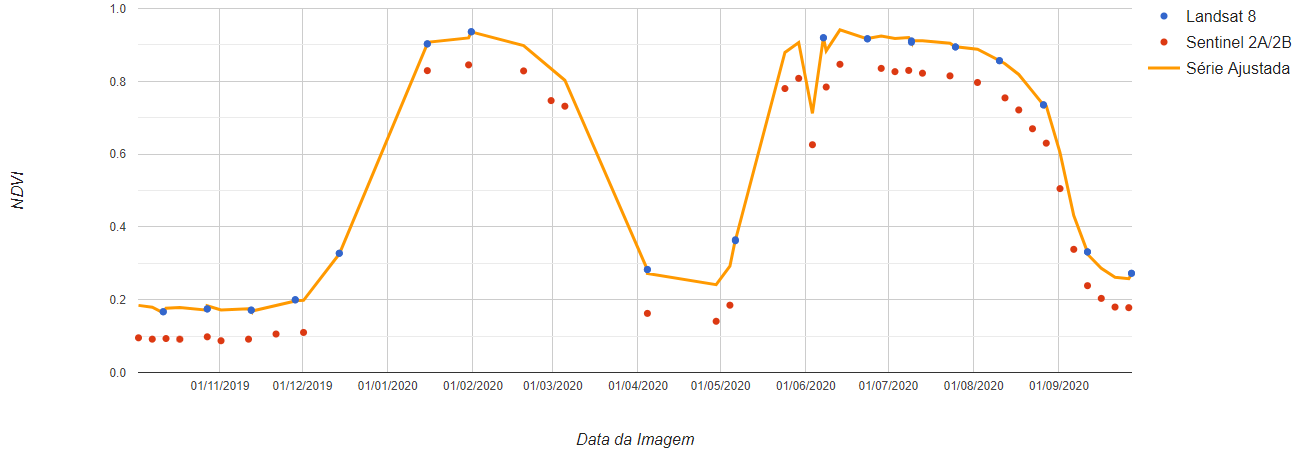
\includegraphics[width=0.7\textwidth]{figuras/serie_temporal_ajustada.png}
\label{fig:correcao_brdf}
\end{figure}


\section{Função de distribuição de reflectância bidirecional}

As imagens adquiridas através de sensores ópticos são suscetíveis as variações dos ângulos (zenital e azimutal) do Sol no momento da captura da imagem, assim como também ao próprio ângulo de visada do sensor, que podem gerar alteração no sombreamento da vegetação e superfície do solo e comprometer a qualidade final da imagem \cite{hadjimitsis2010atmospheric}. A correção dessa interferência na captura da imagem pode ser feita a partir da técnica de BRDF (\textit{Bidirectional Reflectance Distribution Function}) \cite{schaaf2002first}. Neste trabalho, aplicamos esta correção nas imagens utilizando a abordagem proposta por \citeonline{roy2016general}. Na Figura \ref{fig:correcao_brdf} apresentamos o efeito da correção BRDF aplicada em duas imagens que apresentam o efeito da iluminação do sol. 

\begin{figure}[H]
\caption{Efeito da correção da iluminação utilizando a função de distribuição de reflectância bidirecional - BRDF (b) aplicado nas imagens LC08\_178059\_20160130 e LC08\_179059\_20160206 originais (a) adquiridas pelo satélite Landsat 8, sensor OLI, na composição falsa cor (NIR, SWIR1, red).}
\label{fig:correcao_brdf}
\centering
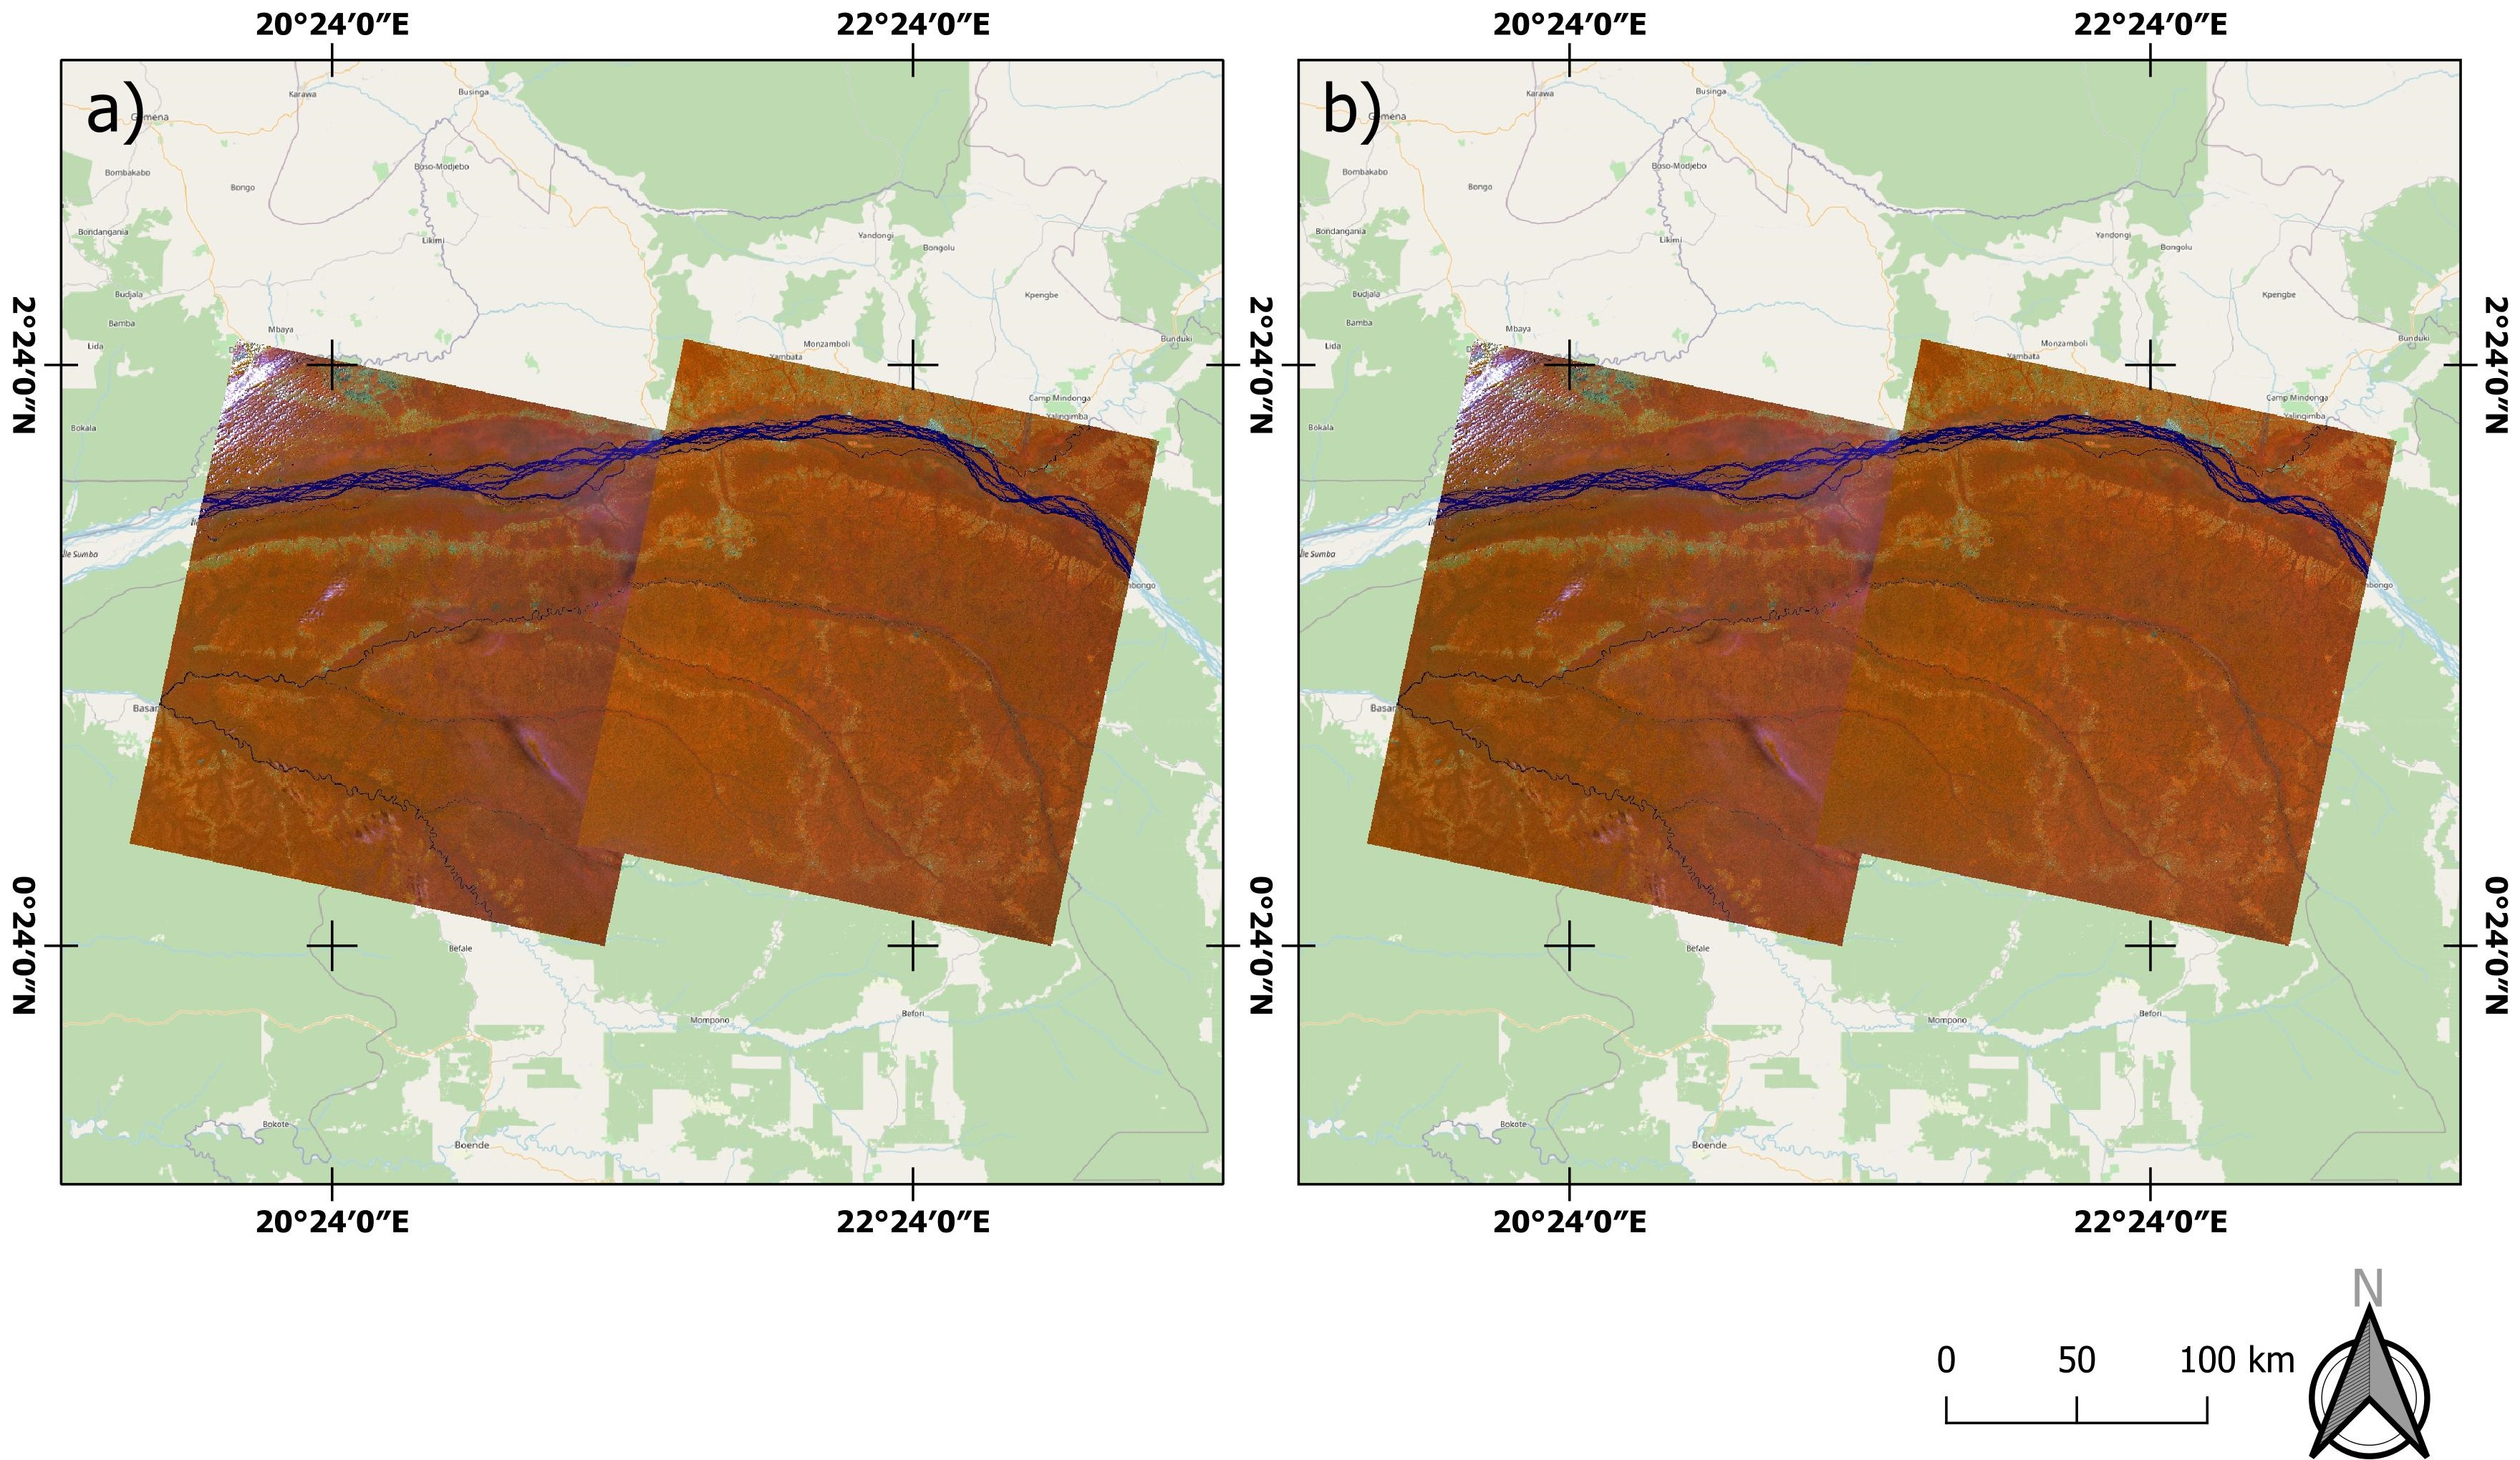
\includegraphics[width=0.6\textwidth]{figuras/aplicacao_brdf.jpg}
\end{figure}

\section{Iluminação do Terreno}

Além do efeito provocado pela variação dos ângulos do sol e do ângulo de visada do sensor, explicados na seção anterior, há também variações de iluminação provocadas pela topografia do terreno, que podem alterar o valor de reflectância do \textit{pixel}, efeito que pode se acentuar com a baixa elevação do sol e superfícies mais ásperas, como montanhas e áreas com alta declividade. 

Para realizarmos a correção da iluminação do terreno, utilizamos a implementação feita por \citeonline{poortinga2019mapping} baseada na abordagem proposta por \citeonline{soenen2005scs}. Nesta correção, utilizamos o modelo digital de elevação, produzido pela \textit{Shuttle Radar Topography Mission} - SRTM \cite{farr2007shuttle}, para obter a declividade e o aspecto da superfície do terreno e os valores contidos nos metadados da imagem referentes aos ângulos zenital e azimutal do sol no momento da captura da imagem. A Figura \ref{fig:correcao_iluminacao_terrano} apresenta um exemplo do efeito da correção em uma imagem de satélite. 

\begin{figure}[H]
\caption{Efeito da correção da iluminação do terreno (b)  aplicado em um recorte da imagem S2A\_MSIL1C\_20210703T132241\_N0301\_R038\_T23LLF\_20210703T164601 (a) adquirida pelo satélite Sentinel 2A, sensor MSI, na composição falsa cor (NIR, SWIR1, RED)}
\label{fig:correcao_iluminacao_terrano}
\centering
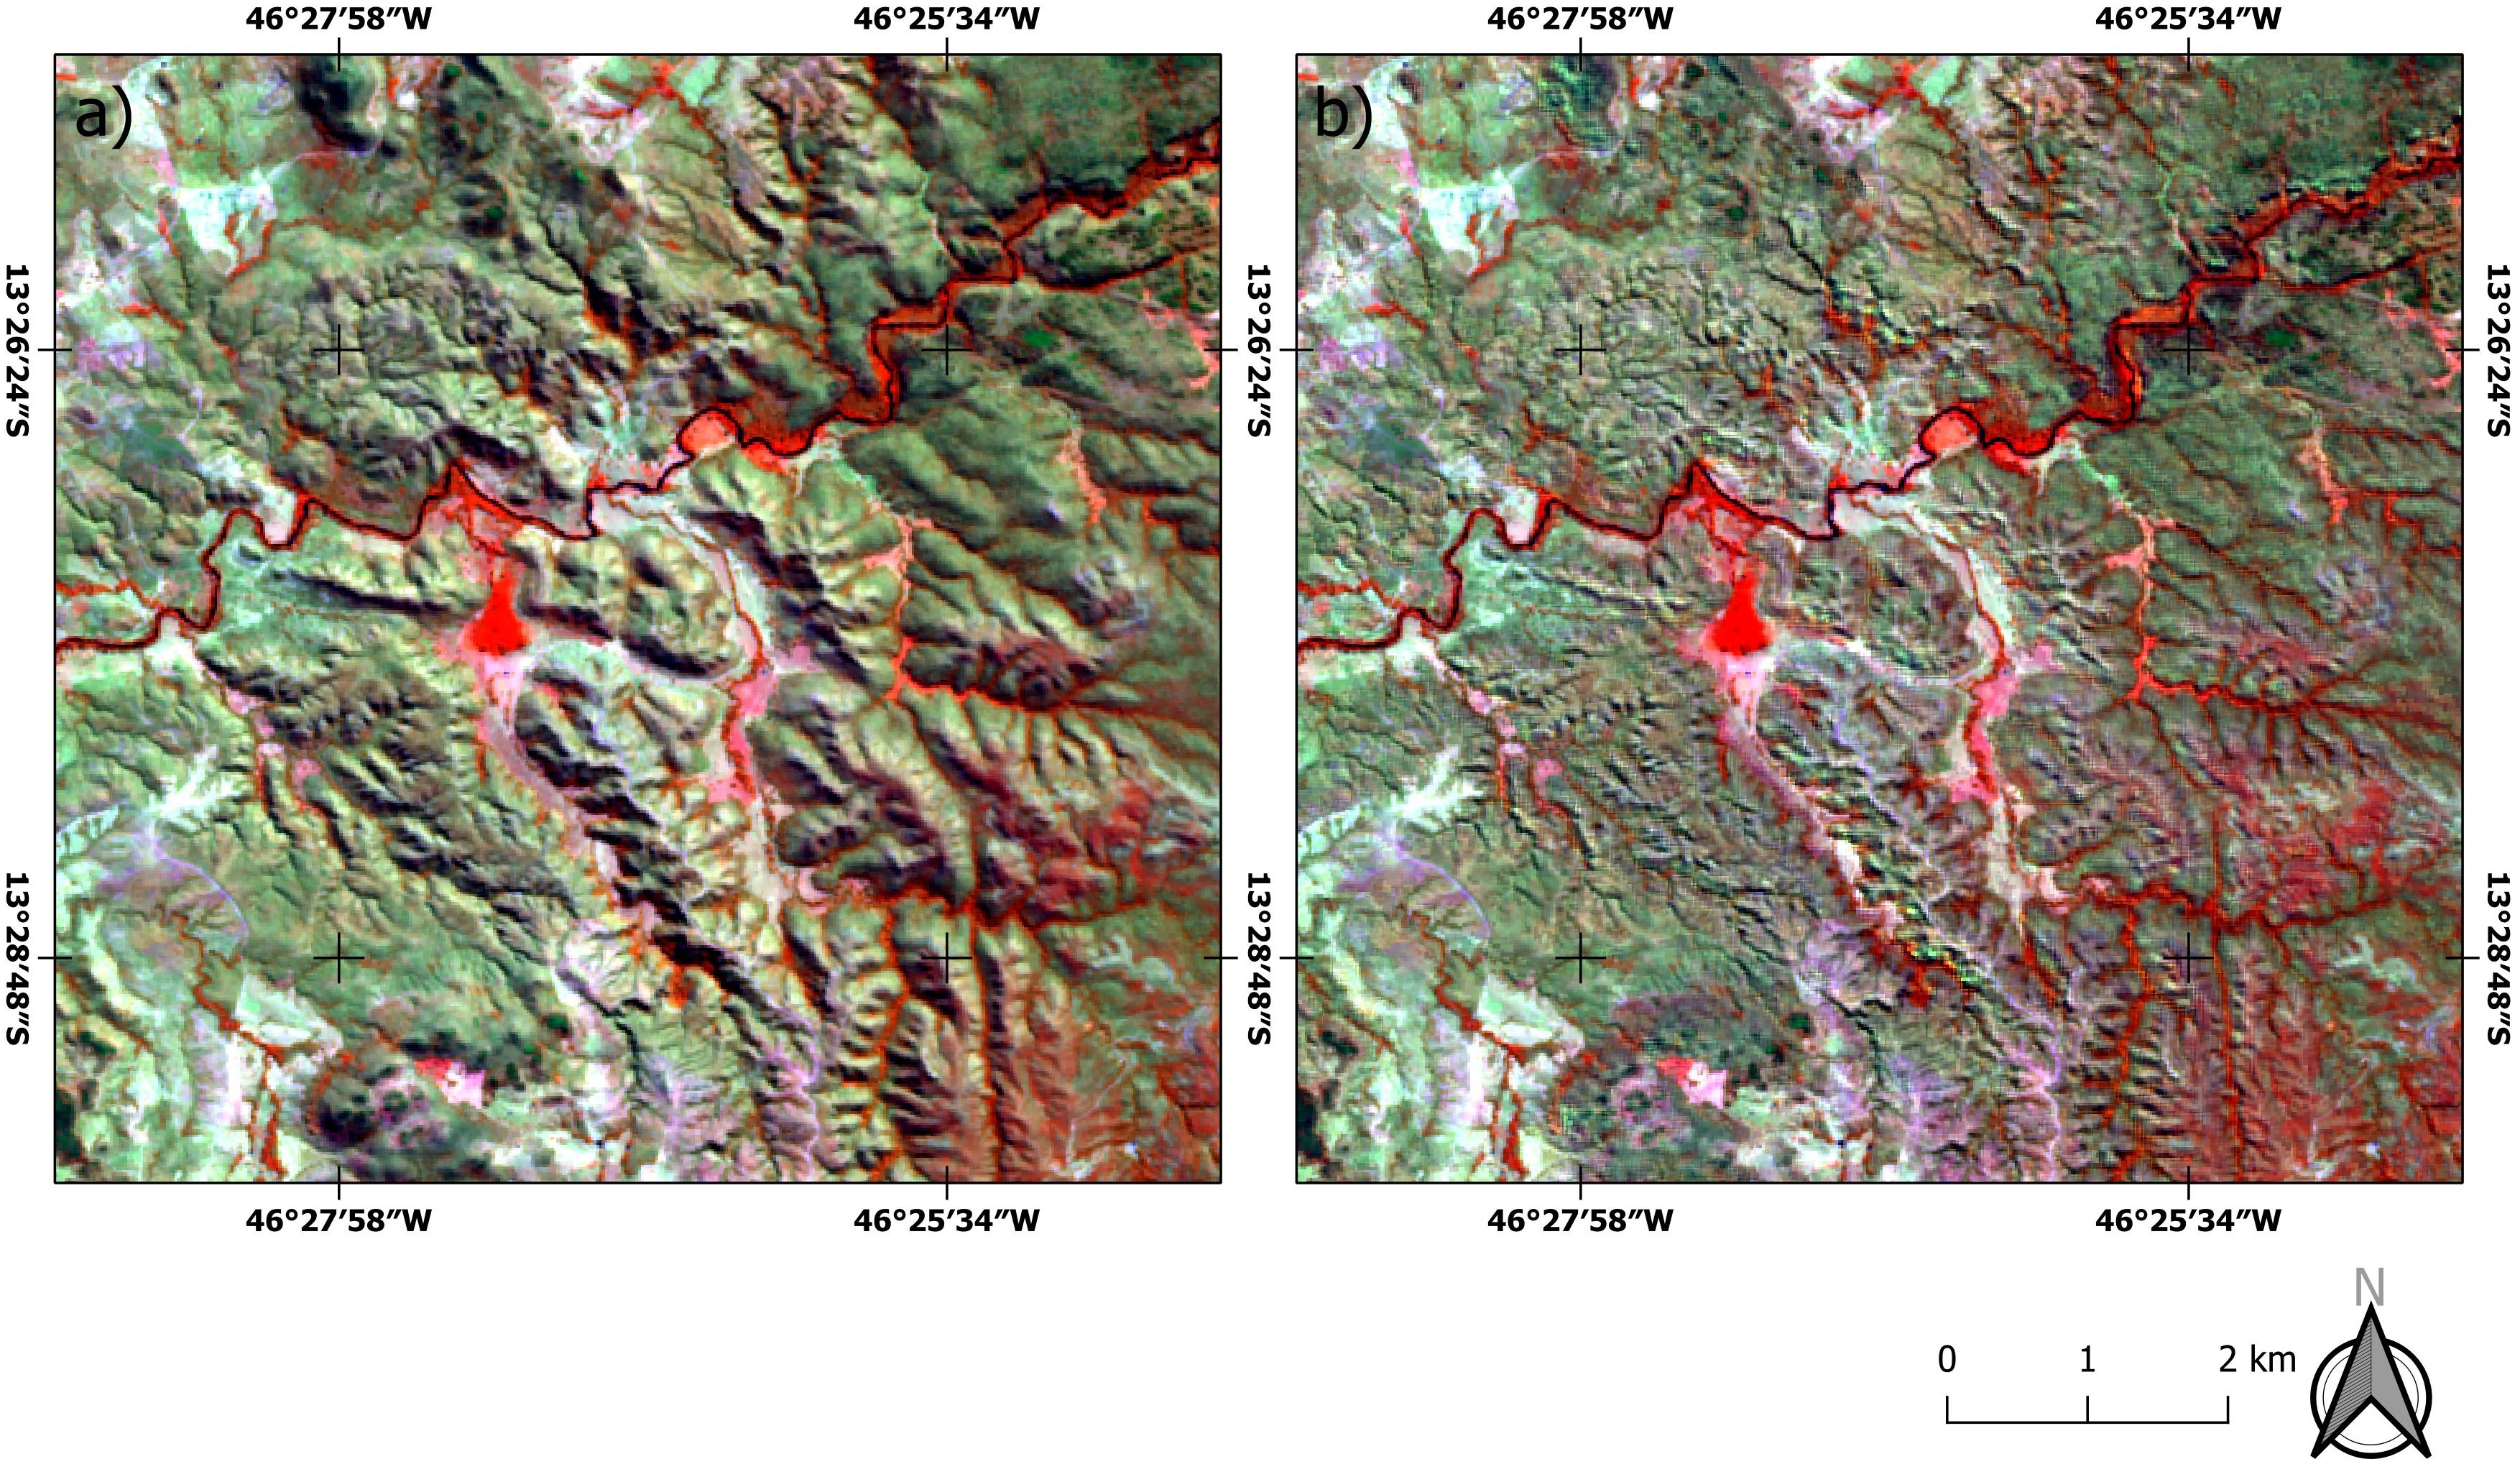
\includegraphics[width=0.6\textwidth]{figuras/aplicacao_correcao_terreno.jpg}
\end{figure}

\section{Máscara de nuvens e sombra de nuvens}

Nuvens e sombra de nuvens podem afetar significativamente sensores ópticos como Landsat 8 OLI e Sentinel 2 MSI,  pois obstruem a visão do sensor e impedem que seja possível visualizar, nas imagens, os alvos em campo como a vegetação, agricultura, pastagem e etc. Dito isso, uma das etapas que realizamos no tratamento das imagens foi remover as nuvens e sombra de nuvens das imagens e deixar apenas \textit{pixels} livres de nuvens e sombra de nuvens (Figura \ref{fig:remocao_nuvens}).  

Para remover as nuvens e sombra de nuvem no Landsat 8, utilizamos a banda de qualidade (QA\_pixel) presente nas imagens de satélite. A banda de qualidade contém estatísticas de qualidade coletadas dos dados da imagem e informações da máscara de nuvem para cada imagem. As imagens dos satélites Sentinel 2A e 2B também possuem uma banda de qualidade indicando os \textit{pixels} de nuvens, porém com uma qualidade muito inferir a banda de qualidade disponível no Landsat 8. A qualidade inferior na detecção de nuvens dos satélites Sentinel 2A e 2B se deve ao fato de que o sensor MSI, presente nos dois satélites, não possui a capacidade de capturar na faixa do infravermelho de ondas longas, também conhecido como banda de temperatura ou banda do termal, essencial para a detecção de nuvens e sombra de nuvens. Como alternativa à banda de qualidade, a ESA lançou uma coleção de imagens que contem, para cada imagem Sentinel 2A/2B, uma imagem com uma única banda em cada \textit{pixel} representa a probabilidade, de 0 à 100, daquele pixel ser nuvem na imagem do satélite original. Essa coleção extra com essas máscaras de probabilidade de nuvem utilizam o algoritmo \textit{s2cloudless} \cite{zupancimproving}. 

\begin{figure}[H]
\caption{Exemplo do processo de identificação de nuvens e sombra de nuvens (áreas amarelas em (b) ) e sua remoção das imagens (áreas com dado nulos, ou cor branca, em (c) ) aplicado em um recorte da imagem LC08\_220069\_20210101 (a) adquirida pelo satélite Landsat 8, sensor OLI, na composição falsa cor (NIR, SWIR1, red).}
\label{fig:remocao_nuvens}
\centering
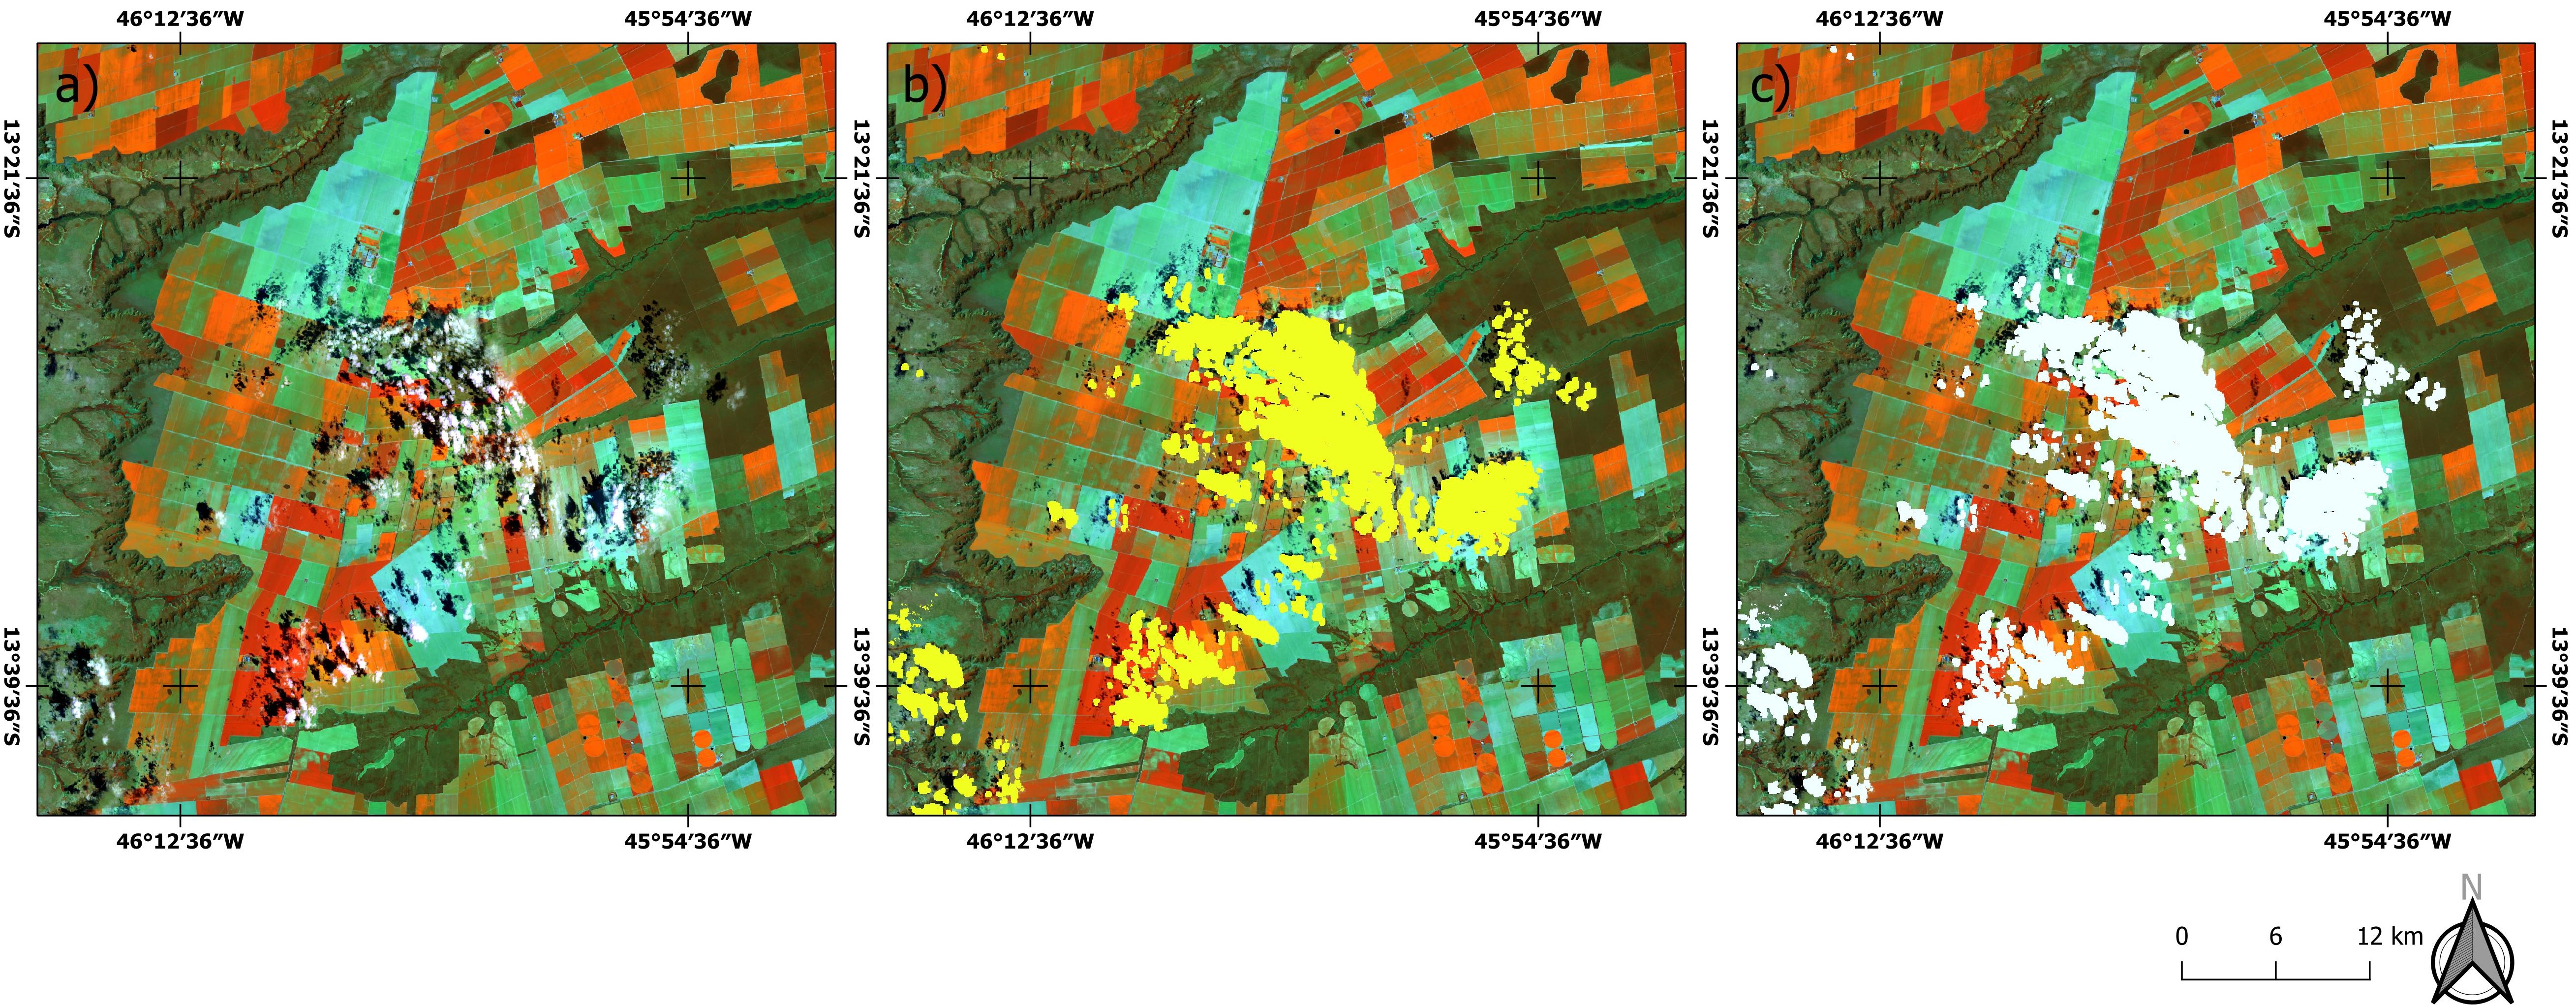
\includegraphics[width=0.8\textwidth]{figuras/mascara_nuvens.jpg}
\end{figure}

\section{Suavização das séries temporais}
\label{sec:suavizacao_series_temporais}

Mesmo com o processo de remoção de nuvens e sombra de nuvens que foi aplicado nas imagens, ainda é possível que existam resquícios de nuvens e sombra de nuvens que não foram apagadas e isso pode afetar os valores de reflectâncias das bandas das imagens e índices de vegetação utilizados. Para diminuir o efeito desses ruídos, aplicamos uma média móvel considerando a junção das duas coleções de imagens, Landsat 8 e Sentinel 2A/2B, e uma janela móvel com tamanho de 16 dias (Figura \ref{fig:serie_ajustada_com_media_movel}).

\begin{figure}[H]
\caption{Exemplo do efeito da suavização da série temporal para um ponto localizado nas coordenadas -45,739369 e -12,156452 (lon, lat) para o período de 01/10/2019 à 01/10/2020. }
\label{fig:serie_ajustada_com_media_movel}
\centering
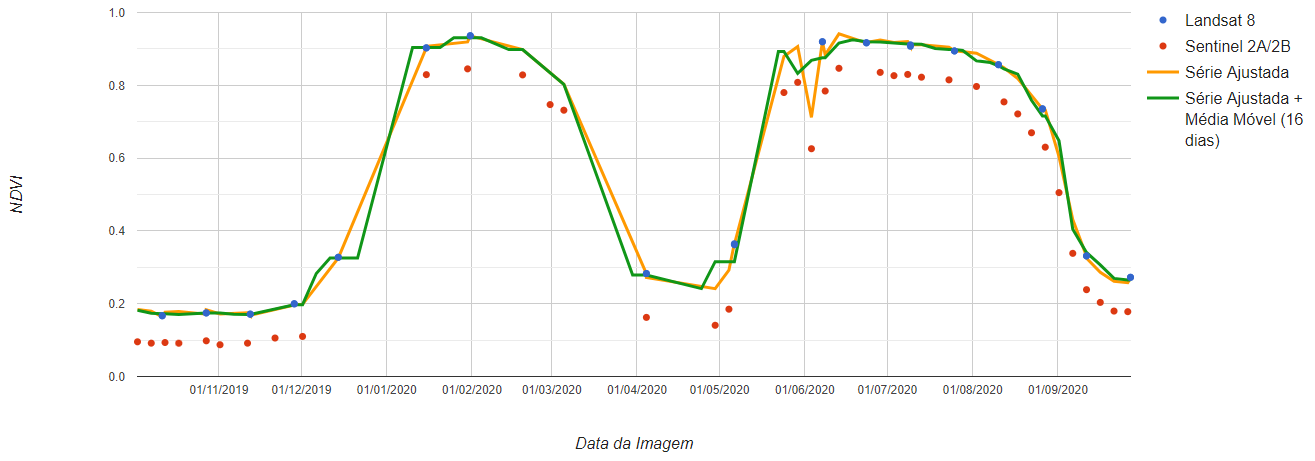
\includegraphics[width=0.7\textwidth]{figuras/serie_temporal_ajustada_media_movel.png}
\end{figure}

\section{Geração dos produtos a cada 16 dias}

A etapa final do processamento das imagens foi uma agregação temporal das imagens individuais em composições de 16 dias. O intervalo de composição foi selecionado correspondente aos produtos de dados MODIS Nível 3. O uso de um intervalo de 16 dias reduz o requisitos para download, armazenamento e processamento de dados em comparação com as imagens individuais que podem ter uma cadência de até 3 dias. Ao longo do ano, foram gerados 23 produtos que foram utilizados para o treinamento e classificação dos modelos. % (Tabela \ref{tab:produtos_16_dias}).

% \begin{table}[H]
% \caption{Dia do ano (DOY) de início e fim para os intervalos de composição dos produtos de 16 dias.}
% \label{tab:produtos_16_dias}
% \centering
% \begin{adjustbox}{width=0.5\textwidth}
% \begin{tabular}{|l|l|l|llll}
% \cline{1-3} \cline{5-7}
% \textbf{Id produto} & \textbf{DOY inicial} & \textbf{DOY final} & \multicolumn{1}{l|}{} & \multicolumn{1}{l|}{\textbf{Id produto}} & \multicolumn{1}{l|}{\textbf{DOY inicial}} & \multicolumn{1}{l|}{\textbf{DOY final}} \\ \cline{1-3} \cline{5-7} 
% 1                   & 1                           & 16                        & \multicolumn{1}{l|}{} & \multicolumn{1}{l|}{13}                  & \multicolumn{1}{l|}{193}                         & \multicolumn{1}{l|}{208}                       \\ \cline{1-3} \cline{5-7} 
% 2                   & 17                          & 32                        & \multicolumn{1}{l|}{} & \multicolumn{1}{l|}{14}                  & \multicolumn{1}{l|}{209}                         & \multicolumn{1}{l|}{224}                       \\ \cline{1-3} \cline{5-7} 
% 3                   & 33                          & 48                        & \multicolumn{1}{l|}{} & \multicolumn{1}{l|}{15}                  & \multicolumn{1}{l|}{225}                         & \multicolumn{1}{l|}{240}                       \\ \cline{1-3} \cline{5-7} 
% 4                   & 49                          & 64                        & \multicolumn{1}{l|}{} & \multicolumn{1}{l|}{16}                  & \multicolumn{1}{l|}{241}                         & \multicolumn{1}{l|}{256}                       \\ \cline{1-3} \cline{5-7} 
% 5                   & 65                          & 80                        & \multicolumn{1}{l|}{} & \multicolumn{1}{l|}{17}                  & \multicolumn{1}{l|}{257}                         & \multicolumn{1}{l|}{272}                       \\ \cline{1-3} \cline{5-7} 
% 6                   & 81                          & 96                        & \multicolumn{1}{l|}{} & \multicolumn{1}{l|}{18}                  & \multicolumn{1}{l|}{273}                         & \multicolumn{1}{l|}{288}                       \\ \cline{1-3} \cline{5-7} 
% 7                   & 97                          & 112                       & \multicolumn{1}{l|}{} & \multicolumn{1}{l|}{19}                  & \multicolumn{1}{l|}{289}                         & \multicolumn{1}{l|}{304}                       \\ \cline{1-3} \cline{5-7} 
% 8                   & 113                         & 128                       & \multicolumn{1}{l|}{} & \multicolumn{1}{l|}{20}                  & \multicolumn{1}{l|}{305}                         & \multicolumn{1}{l|}{320}                       \\ \cline{1-3} \cline{5-7} 
% 9                   & 129                         & 144                       & \multicolumn{1}{l|}{} & \multicolumn{1}{l|}{21}                  & \multicolumn{1}{l|}{321}                         & \multicolumn{1}{l|}{336}                       \\ \cline{1-3} \cline{5-7} 
% 10                  & 145                         & 160                       & \multicolumn{1}{l|}{} & \multicolumn{1}{l|}{22}                  & \multicolumn{1}{l|}{337}                         & \multicolumn{1}{l|}{352}                       \\ \cline{1-3} \cline{5-7} 
% 11                  & 161                         & 176                       & \multicolumn{1}{l|}{} & \multicolumn{1}{l|}{23}                  & \multicolumn{1}{l|}{353}                         & \multicolumn{1}{l|}{365 (366)}                 \\ \cline{1-3} \cline{5-7} 
% 12                  & 177                         & 192                       &                       &                                          &                                                  &                                                \\ \cline{1-3}
% \end{tabular}
% \end{adjustbox}
% \end{table}

\section{Padronização das classes utilizadas para o treinamento dos modelos}

Os polígonos disponíveis nos dados de referência foram coletados em trabalhos de campo e contém um conjunto de classes de uso e cobertura da terra que foram definidos pelos analistas. Das classes definidas, algumas possuem poucas amostras, enquanto outras possuem uma definição de classe que não compreende uma categoria de uso e cobertura da terra, como a classe "not identified". Neste trabalho, focamos nossos esforços no desenvolvimento de uma metodologia de mapeamento do uso e cobertura da terra que busca mapear as classes mais representativas e consistentes do conjunto de dados original. Para isso, removemos e agregamos algumas classes disponíveis no conjunto original e geramos um novo conjunto com treze classes de uso e cobertura (Tabela \ref{tab:classes_remapeadas}) que possui as classes mais representativas e consistentes do conjunto de dados original. 

% https://code.earthengine.google.com/bbc8502f24f5b562213c9cac88444bec

\definecolor{soybean}{rgb}{255, 227, 46}

\begin{table}[H]
\caption{Classes originais presentes nos dados de referência e sua classe correspondente na nova legenda que foi criada para simplificar a lista de classes que foram mapeadas neste trabalho.}
\label{tab:classes_remapeadas}
\centering
\begin{adjustbox}{width=0.5\textwidth}
\begin{tabular}{|l|l|l|l|l|}
\hline
\textbf{Classe original}   & \textbf{Quantidade de Polígonos} & \textbf{Id da nova classe} & \textbf{Nome da nova classe} \\ \hline
not identified    & 763                     & --                & --                 \\ \hline
soybean           & 4743                    & 1                 & soybean            \\ \hline
maize             & 430                     & 2                 & maize              \\ \hline
corn              & 1168                    & 2                 & maize              \\ \hline
cotton            & 1077                    & 3                 & cotton             \\ \hline
coffee            & 439                     & 4                 & coffee             \\ \hline
beans             & 149                     & 5                 & beans              \\ \hline
wheat             & 3                       & --                & --                 \\ \hline
sorghum           & 706                     & 6                 & sorghum            \\ \hline
millet            & 1754                    & 7                 & millet             \\ \hline
eucalyptus        & 415                     & 8                 & eucalyptus         \\ \hline
pasture           & 1516                    & 9                 & pasture            \\ \hline
hay               & 409                     & 10                & hay                \\ \hline
grass             & 280                     & 11                & grass              \\ \hline
crotalari         & 2                       & --                & --                 \\ \hline
crotalaria        & 7                       & --                & --                 \\ \hline
maize+crotalari   & 4                       & --                & --                 \\ \hline
cerrado           & 2630                    & 12                & natural vegetation \\ \hline
conversion area   & 346                     & 13                & exposed soil       \\ \hline
uncultivated soil & 14673                   & 13                & exposed soil       \\ \hline
ncc               & 24                      & --                & --                 \\ \hline
brachiaria        & 1032                    & --                & --                 \\ \hline     
\end{tabular}
\end{adjustbox}
\end{table}

\section{Geração dos pontos que foram usados para obter as séries temporais}

Os dados que temos no LEM e LEM+ dataset são polígonos anotados ao longo do tempo com as diferentes classes de uso e cobertura. Para aumentarmos a nossa quantidade de amostras e incrementar a variabilidade espectral das classes definidas, realizamos o sorteio aleatório simples de pontos dentro dos polígonos e cruzamos as coordenadas dos pontos com as imagens de satélite para obter as séries temporais que foram utilizadas para o treinamento, validação e teste dos modelos. Ao todo, geramos 79990 pontos e obtemos, consequentemente, 79990 séries temporais, cada série temporal associada à um único ponto. 

\section{Remoção de dados nulos}

Após a remoção das nuvens e sombra de nuvens, realizamos uma etapa de suavização da série temporal de imagens (Seção \ref{sec:suavizacao_series_temporais}) que preencheu parte dos dados nulos deixados pela etapa de remoção de nuvens e sombra de nuvens. Para os dados nulos restantes, cerca de 13\% de todo o nosso conjunto de dados, realizamos a remoção. 

\renewcommand{\cleardoublepage}{}
\renewcommand{\clearpage}{}
\vspace{5mm}
\chapter{Análise Exploratória dos Dados e Análise com Modelos de Aprendizado de Máquina}

\section{Distribuição das classes}

Durante nossa análise exploratória, o primeiro passo foi verificar a distribuição da ocorrência das classes no conjunto de dados. Ao calcularmos a distribuição das classes (Figura \ref{fig:distribuicao_classes}) constatamos uma grande desproporção entre as classes. Por exemplo, apenas a classe 'exposed\_soil' representa quase a metade de todo o conjunto de dados. A abundância de exemplos dessas classes majoritárias ('exposed\_soil', 'soybean', 'natural\_vegetation', e etc) pode inundar as classes minoritárias ('eucalyptus', 'grass', 'beans', e etc). A maioria dos algoritmos de aprendizado de máquina para classificação são projetados e demonstrados em problemas que assumem uma distribuição igual de classes. Isso significa que uma aplicação de um modelo pode focar em aprender apenas as características das observações abundantes, negligenciando os exemplos das classes minoritárias.

\begin{figure}[H]
\caption{Distribuição da ocorrência das classes em todo o conjunto de dados.}
\label{fig:distribuicao_classes}
\centering
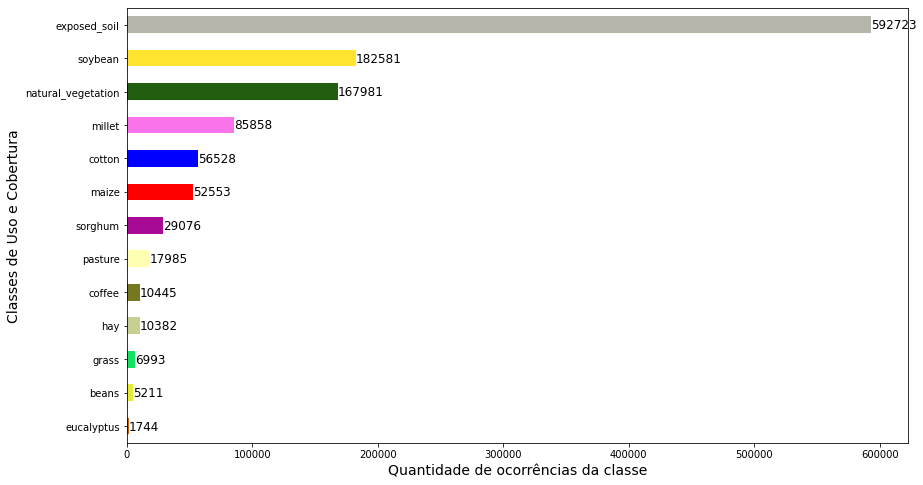
\includegraphics[width=0.6\textwidth]{figuras/ocorrencia_das_classes.png}
\end{figure}


\section{Visualização das \textit{features} nas séries temporais}

Após analisarmos a proporção das classes no conjunto de dados, o próximo passo foi visualizar o comportamento das \textit{features} nas séries temporais. Ao analisar as \textit{features} nas séries temporais, é possível identificarmos o comportamento que cada \textit{feature} tem com a mudança da classe de uso e cobertura. Por exemplo, na Figura \ref{fig:features_na_serie_temporal} é possível identificarmos que na classe 'soybean', a \textit{feature} 'RED' tende a ter valores menores e a \textit{feature} 'NIR' tende a ter valores maiores, em comparação com a classe 'exposed\_soil'. Também é possível identificarmos que a \textit{feature} 'NDVI', gerada a partir das diferença normalizada das \textit{features} 'NIR' e 'RED' tente a ter valores mais altos na classe 'soybean' do que na classe 'exposed\_soil', o que indica que essa \textit{feature} pode ser usada pelo algoritmos para diferenciar essas duas classes.

\begin{figure}[H]
\caption{Exemplo de uma série temporal com as \textit{features} utilizadas para o treinamento dos modelos e suas classes de uso e cobertura da terra correspondentes ao longo do tempo.}
\label{fig:features_na_serie_temporal}
\centering
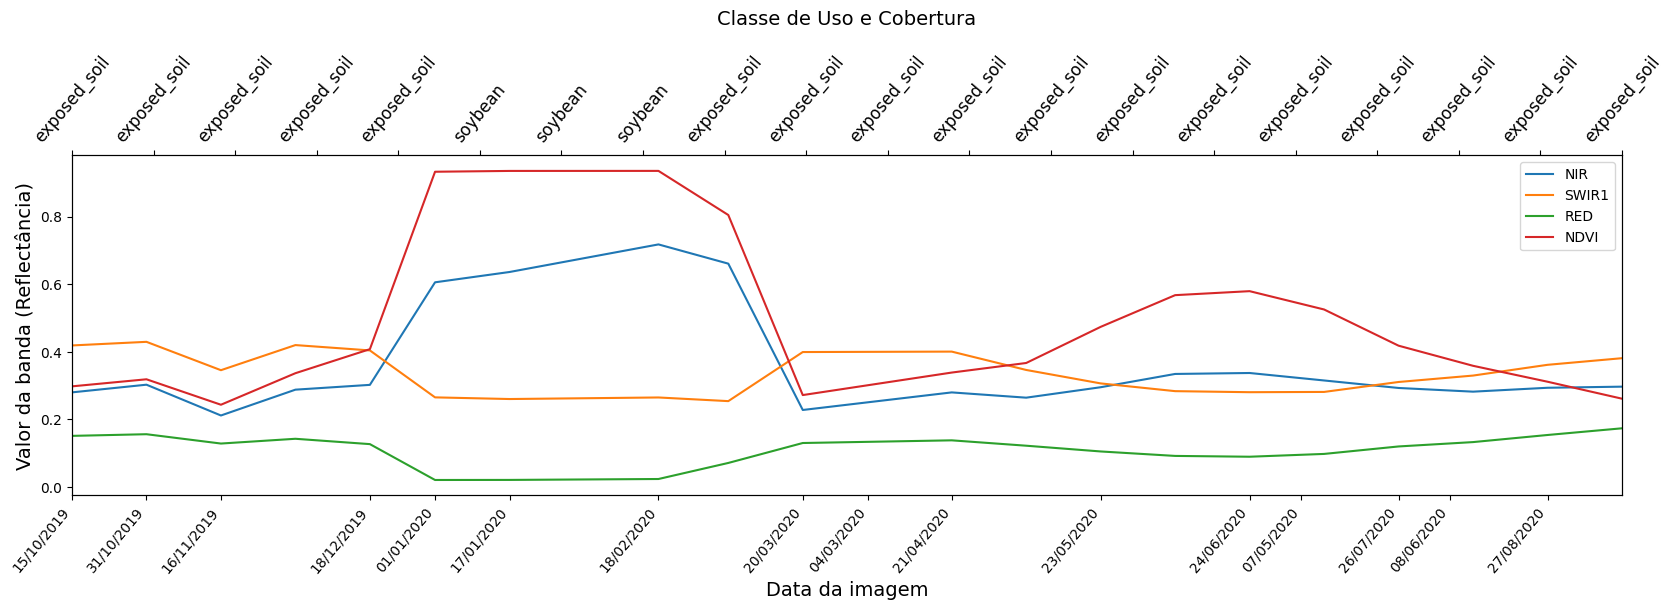
\includegraphics[width=0.8\textwidth]{figuras/serie_temporal_features.png}
\end{figure}

\section{Análise de valores discrepantes nas séries temporais}

Valores discrepantes são valores que diferem significativamente dos padrões e tendências dos outros valores do conjunto de dados. Na geração das séries temporais, utilizamos como referência a classe indicada pelo analista para o respectivo mês daquele produto de imagem de satélite. Como para um único mês temos sempre dois produtos de imagens de satélite, é possível que o analista tenha, por exemplo, indicado que no mês da análise a classe de uso seja um cultivo de soja, porém nas imagens de satélite aquela soja seja visível apenas no primeiro produto do mês, já no segundo produto, após uma eventual colheita no meio do mês, esse produto pode ter sido indicado como cultivo de soja ('soybean'), mas essa área já tenha ficado com o comportamento espectral de solo exposto ('exposed\_soil') após a colheita. Na Figura \ref{fig:boxplot_das_features_com_outliers} é possível identificarmos, através da análise dos diagramas de caixa, que muitas das classes apresentam valores discrepantes. No caso da classe de soja ('soybean'), por exemplo, é esperado que os valores do 'NDVI' fiquem acima de 0,4 \cite{risso2009potencialidade}, porém nos diagramas é possível observarmos que existem observações indicadas como soja com valores de 'NDVI' abaixo de 0,4, indicando, possivelmente, que essas áreas já foram colhidas. 

Para evitarmos que esses valores discrepantes interfiram negativamente nos modelos criados, realizamos a remoção de todas essas observações discrepantes em todas as classes mapeadas. Antes da remoção dos valores discrepantes, haviam 1.523.364 observações em todo o conjunto de dados, após a eliminação dos valores discrepantes restaram 1.384.317 observações, ou seja, uma eliminação de quase 10\% de valores discrepantes.

\begin{figure}[H]
\caption{Distribuição dos valores, por classe de uso e cobertura, das observações em cada uma das \textit{features} utilizadas para treinar os modelos. Nos diagramas, os valores discrepantes não foram removidos.}
\label{fig:boxplot_das_features_com_outliers}
\centering
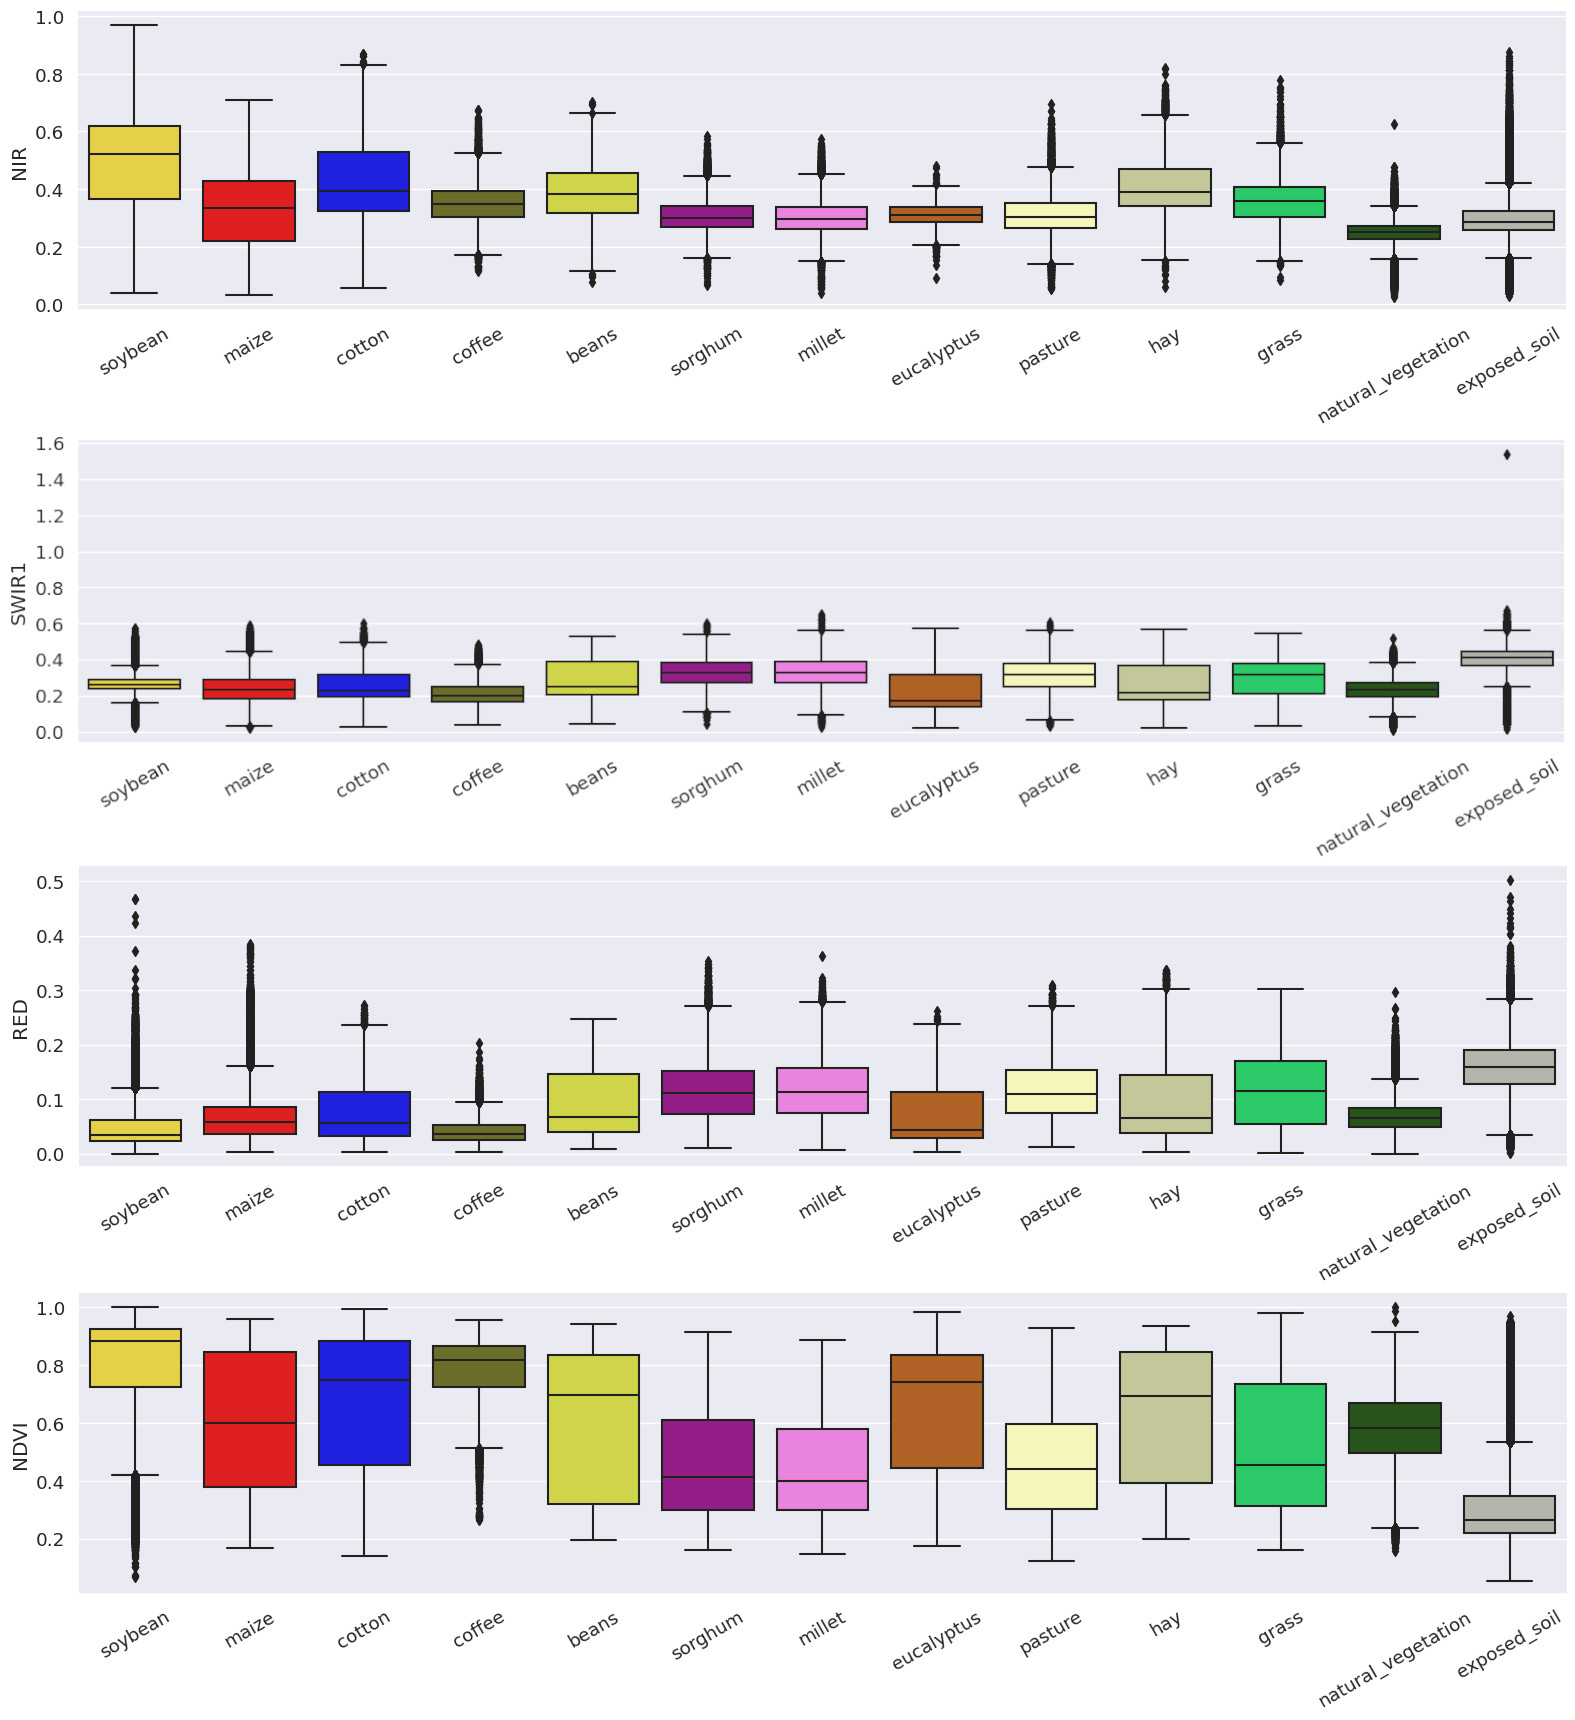
\includegraphics[width=0.6\textwidth]{figuras/catplot_features.jpg}
\end{figure}

\section{Análise da capacidade das \textit{features} em separar as classes de uso e cobertura da terra que foram mapeadas}

Após a eliminação das observações discrepantes, a próxima análise que executamos foi verificar a capacidade de cada uma das \textit{features} de separar determinadas classes de uso e cobertura. Na Figura \ref{fig:analise_confusao_entre_classes_por_feature} é possível verificarmos quais \textit{features} melhor contribuiem para a separação de determinadas classes. Por exemplo, é possível observarmos que as \textit{features} 'RED' e 'NDVI' melhor contribuem para a separação entre as classes 'soybean', 'exposed\_soil' e 'natural\_vegetation'. Nos gráficos é possível observar que, nessas \textit{features}, essas classes possuem uma menor sobreposição entre as curvas, o que indica que um modelo de aprendizado de máquina terá maior facilidade em separar essas classes com essas \textit{features}. Ainda na Figura \ref{fig:analise_confusao_entre_classes_por_feature}, é possível analisarmos se a combinação de duas \textit{features} pode ajudar a separar determinadas classes. Por exemplo, Na combinação entre as \textit{features} ('NIR', 'RED'), ('SWIR1', 'RED'), ('SWIR1', 'NIR'), ('NDVI', 'NIR') e ('NDVI', 'SWIR1) é possível observarmos que os pontos da classe 'soybean' ficam mais agrupados e separados dos demais do que nas outras combinações, o que pode indicar que a combinação dessas \textit{features} pode auxiliar na identificação dessa classe. 

\begin{figure}[H]
\caption{Gráficos com a distribuição dos valores, por classe, para combinações entre as diferentes \textit{features} (gráficos de pontos) e entre a mesma \textit{feature} (gráficos de linhas).}
\label{fig:analise_confusao_entre_classes_por_feature}
\centering
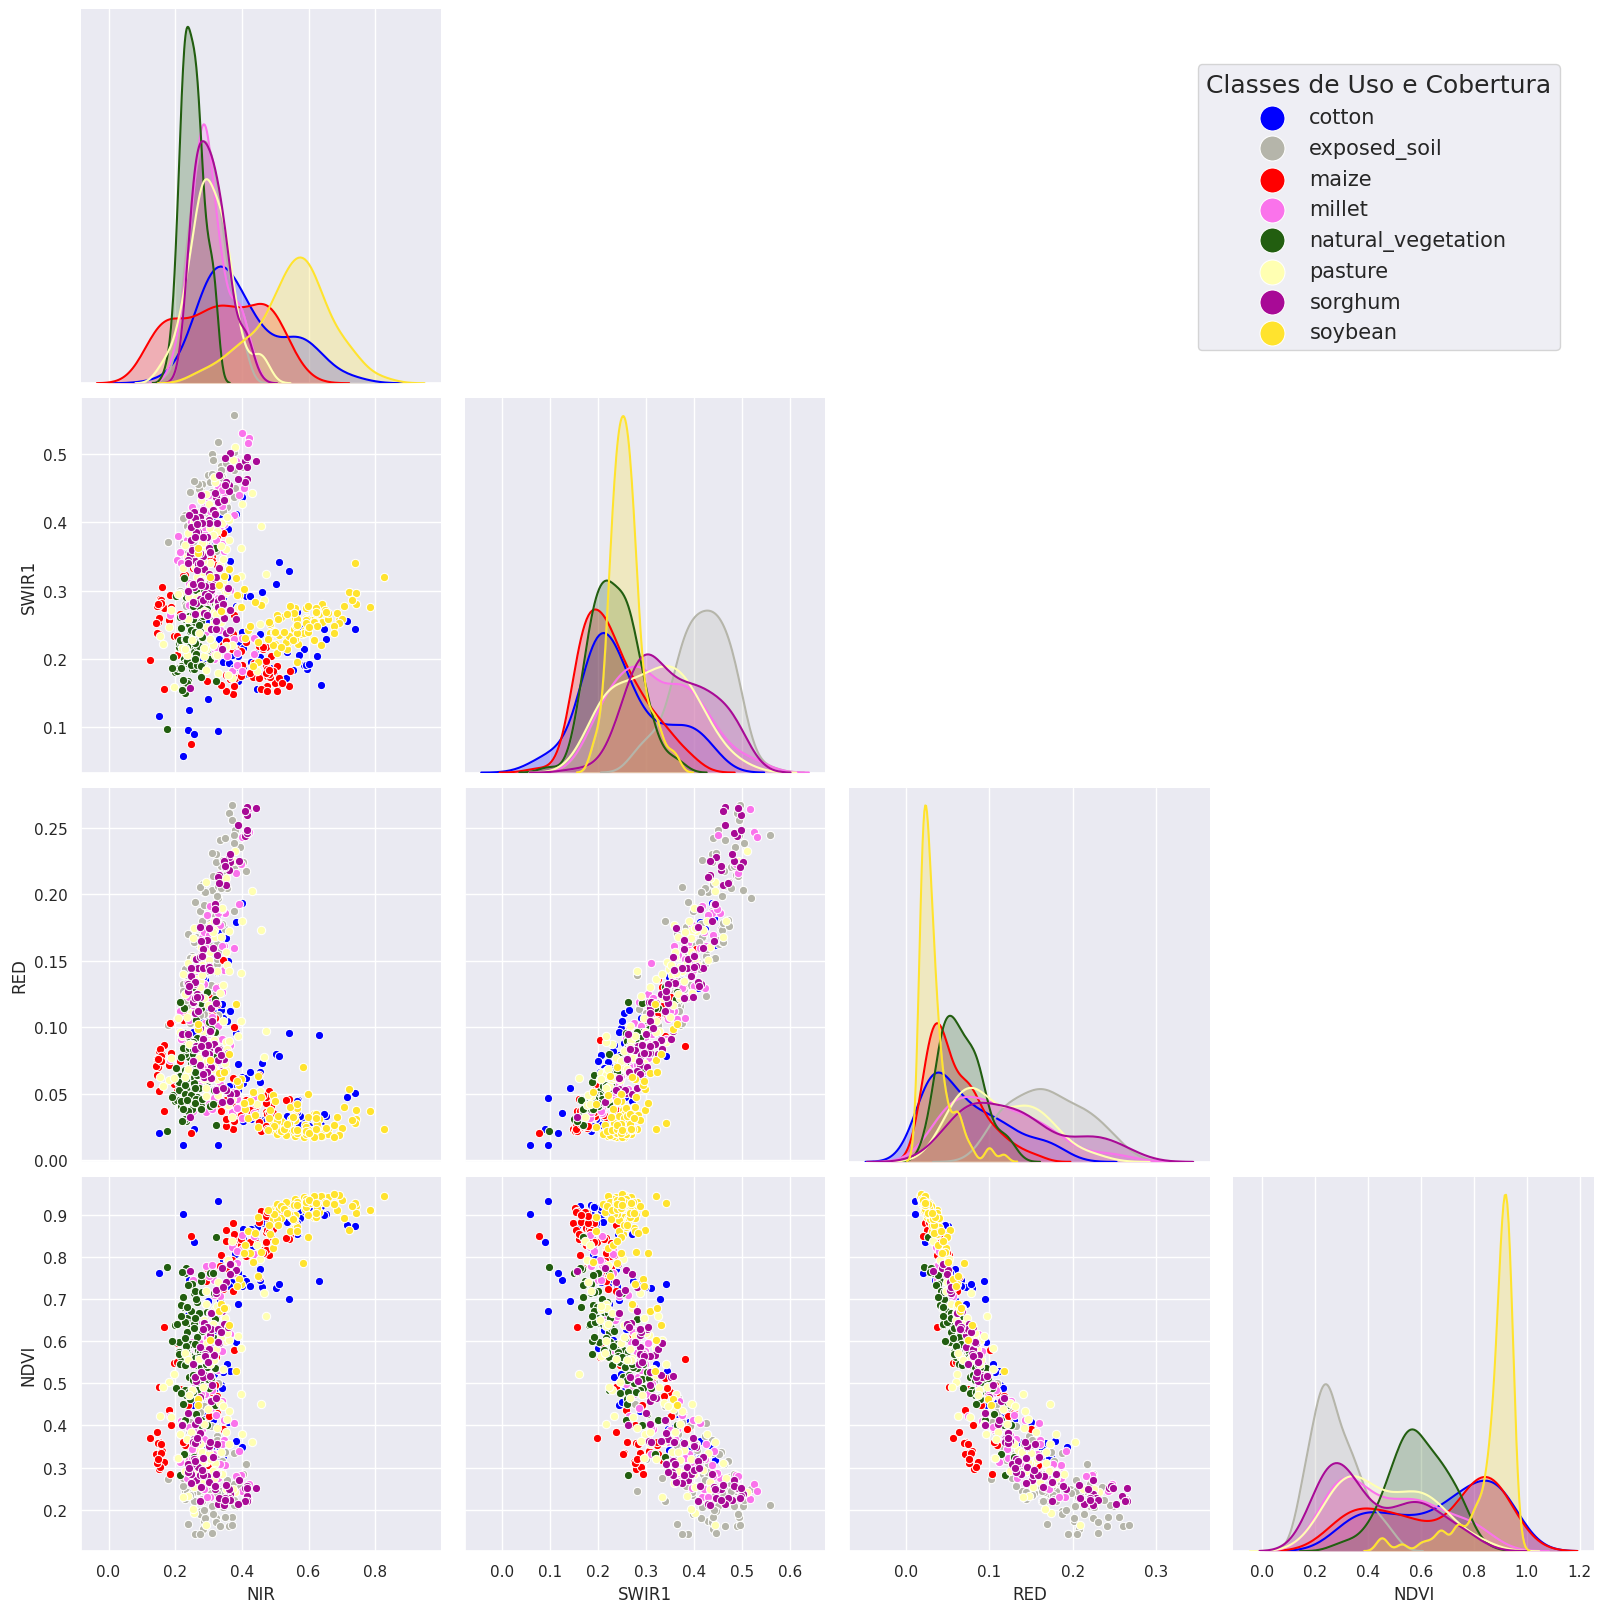
\includegraphics[width=0.5\textwidth]{figuras/correlacao_features_por_classe.png}
\end{figure}

\section{Criação dos modelos de Aprendizado de Máquina}

Neste trabalho, avaliamos três modelos de classificação de uso e cobertura da terra, dois modelos baseado em árvores de decisão utilizando Random Forest \cite{breiman2001random} e um modelo baseado em redes neurais recorrentes utilizando a arquitetura Long Short-Term Memory (LSTM) \cite{hochreiter1997long}.


O Random Forest é um dos algoritmos mais populares para classificação supervisionada  das últimas décadas, sua popularidade é devido, principalmente, às seus ótimos resultados obtidos sem muita parametrização e sem muita necessidade de um grande conjunto de dados de treinamento. 

Rede Neural Recorrente (RNN) é um tipo de Rede Neural onde a saída da etapa anterior é alimentada como entrada para a etapa atual, ou seja, ela possui uma “memória” que guarda todas as informações sobre o que foi calculado. A arquitetura de RNN que utilizamos foi a chamada Long Short-Term Memory - LSTM, uma arquitetura de rede neural recorrente específica que foi projetada para modelar sequências temporais e suas dependências de longo alcance com mais precisão do que RNNs convencionais \cite{sak2014long}, característica importante quando trabalhamos com séries temporais mais longas. 

Para o treinamento e análise da acurácia dos modelos, os dados foram separados em três conjuntos distintos: 80\% treinamento, 10\% validação e 10\% teste. Segundo \citeonline{hastie2009elements}, o conjunto de treinamento deve ser usado para ajustar o modelo; o conjunto de validação deve ser usado para estimar o erro da predição do modelo, e o conjunto de teste deve ser utilizado para a avaliação do erro da generalização do modelo final escolhido. 


\subsection{Modelo Random Forest}

Para a classificação utilizando o Random Forest, utilizamos duas diferentes bibliotecas. A primeira foi a biblioteca scikit-learn, versão 0.24.2, que implementa o Random Forest classico através da classe RandomForestClassifier. Já a segunda foi a biblioteca imbalanced-learn, versão 0.8.1, que implementa uma versão adaptada do Random Forest através da classe BalancedRandomForestClassifier, que aplica um balanceamento entres as classes para dar maior importância as classes minoritárias durante o processo de treinamento do modelo (Figura \ref{fig:parametros_random_forest}). 

\begin{figure}[H]
\centering
\caption{Parâmetros utilizados nos classificadores baseados em Random Forest com e sem o balanceamento das classes.}
\label{fig:parametros_random_forest}
\begin{lstlisting}[language=Python]
# Importando as classes
from sklearn.ensemble import RandomForestClassifier
from imblearn.ensemble import BalancedRandomForestClassifier

# Random Forest sem balanceamento das classes
rf_model = RandomForestClassifier(n_estimators=200, random_state=1, n_jobs=-1)

# Random Forest com balanceamento das classes
brf_model = BalancedRandomForestClassifier(n_estimators=200, random_state=1, n_jobs=-1)

\end{lstlisting}
\end{figure}

\subsection{Modelo LSTM}

Para a construção do modelo LSTM, utilizamos a biblioteca TensorFlow, versão 2.3.0. O modelo que desenvolvemos (Figura \ref{fig:arquitetura_lstm}) utiliza duas camadas LSTM com 128 neurônios cada. Para camada de saída utilizamos uma camada do tipo TimeDistributed com uma camada densamente conectada com a quantidade de neurônios igual a quantidade de classes que queremos mapear. Para ativação da última camada utilizamos a função Softmax. Essa combinação na camada de saída faz com que a saída do modelo seja, para cada ponto da série temporal, uma lista com as probabilidades para cada classe.  Configuramos o modelo para utilizar o otimizador \textit{Adam}, função de perda \textit{categorical\_crossentropy} e como métrica de avaliação a \textit{categorical\_accuracy}, todos parâmetros disponíveis na biblioteca TensorFlow. 

\begin{figure}[H]
\centering
\caption{Arquitetura baseada em LSTM utilizada para a classificação das séries temporais.}
\label{fig:arquitetura_lstm}
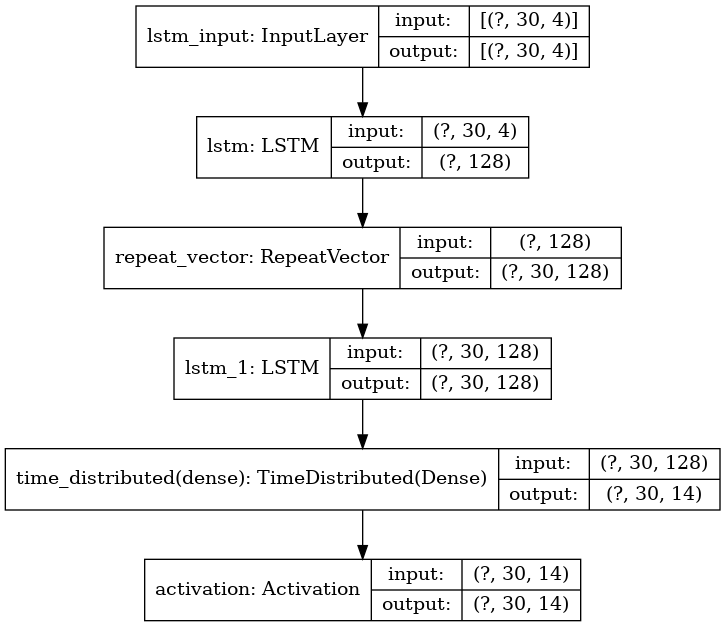
\includegraphics[width=0.4\textwidth]{figuras/lstm.png}
\end{figure}

\renewcommand{\cleardoublepage}{}
\renewcommand{\clearpage}{}
\vspace{5mm}
\chapter{Discussão dos Resultados}

Para avaliarmos a qualidade dos modelos, utilizamos as seguintes métricas: 

\begin{itemize}
    \item Acurácia do produtor (precisão): de todos os elementos de uma classe, quantos por cento, o modelo conseguiu identificar; 
    \item Acurácia do usuário (revocação): de todos os elementos que o modelo identificou como uma determinada classe, quantos por cento, são realmente daquela classe; 
    \item \textit{F1-Score}: é a média harmônica da acurácia do produtor e do usuário. É calculado utilizando a formulá: $\frac{2 * AP * AU}{AP + AU}$, onde AP é a acurácia do produtor e AU é a acurácia do usuário.
\end{itemize}

Na Figura \ref{fig:analise_acuracia}, apresentamos o resultado da análise de acurácia utilizando o conjunto de dados de teste para os três modelos desenvolvidos. Avaliando os resultados, é possível constatarmos que, entre os dois modelos baseados em \textit{Random Forest}, o modelo sem o balanceamento das classes atingiu melhores resultados do que o modelo com balanceamento das classes. Já entre os três modelos desenvolvidos, o modelo baseado em LSTM, que utiliza o contexto de toda a série temporal para a classificação, atingiu os melhores resultados. 

\begin{figure}[H]
\caption{Matrizes de confusão com a análise de acurácia para os modelos: a) \textit{Random Forest} sem balanceamento das classes, b) \textit{Random Forest} com balanceamento das classes e c) modelo baseado na LSTM.}
\label{fig:analise_acuracia}
\centering
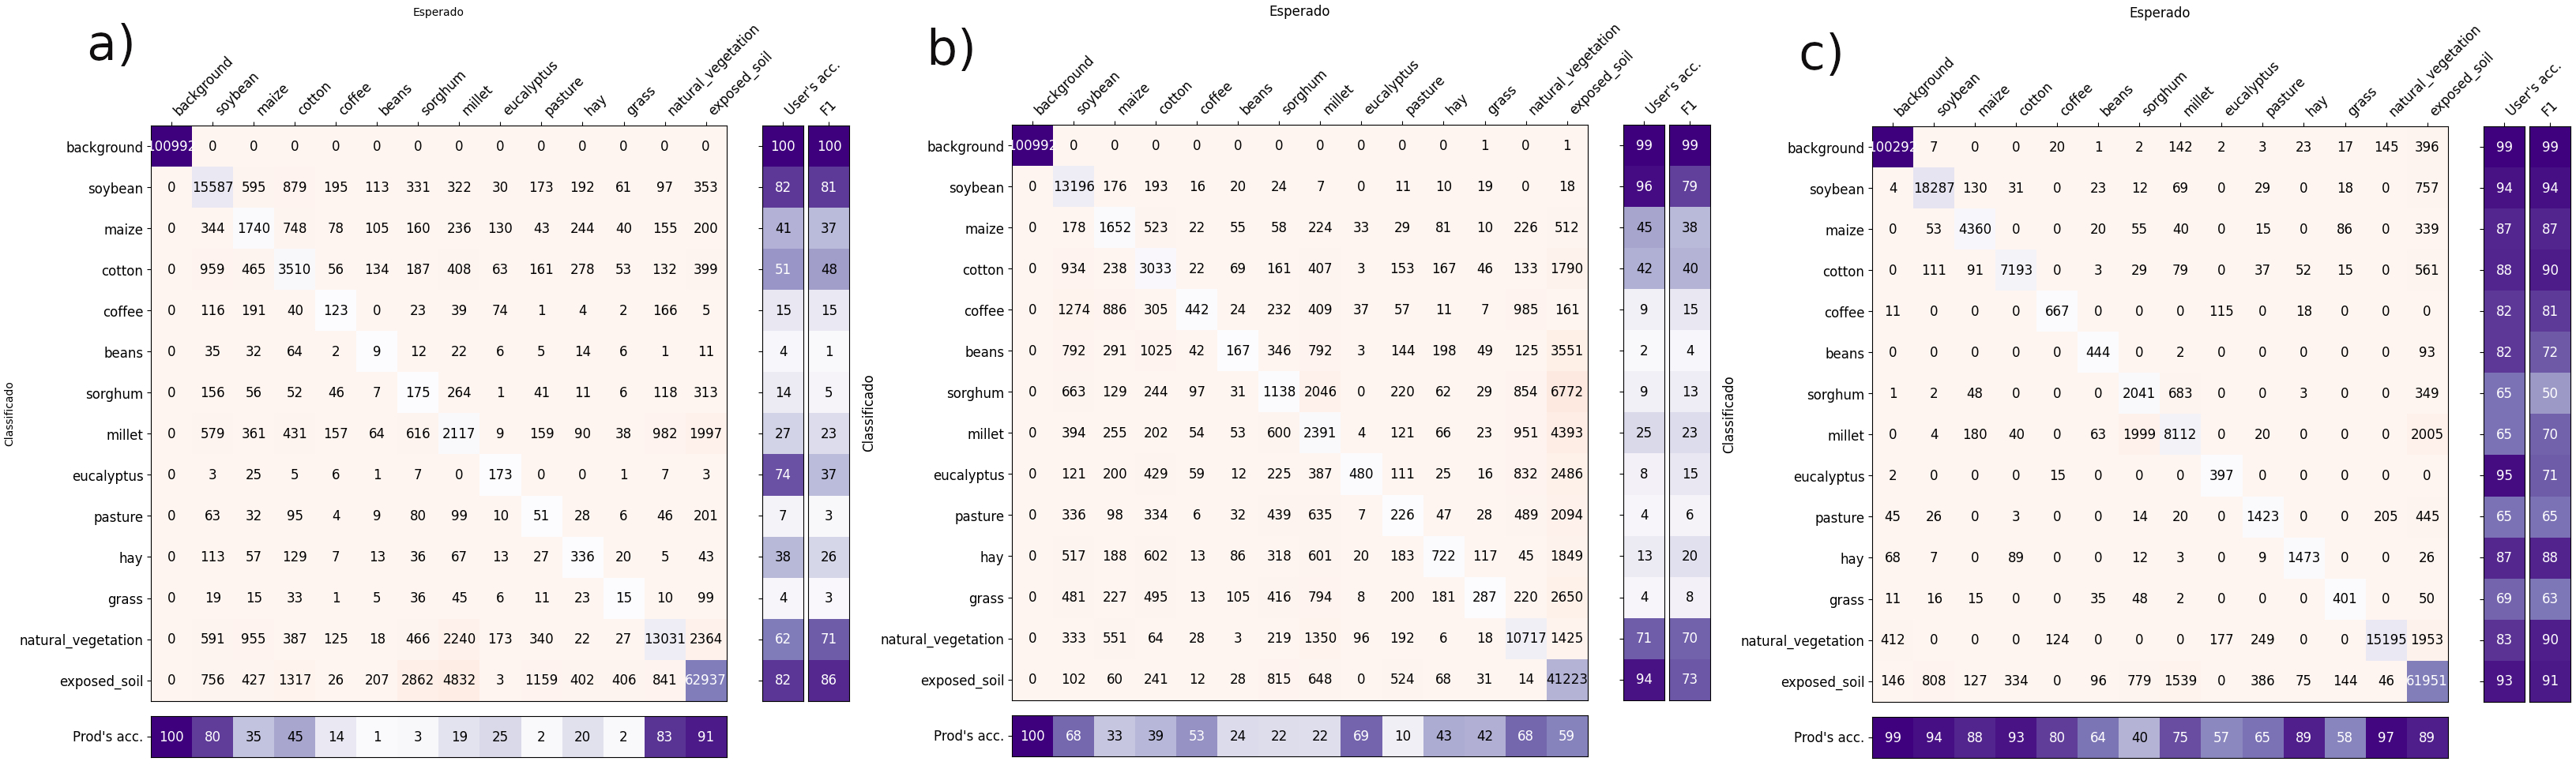
\includegraphics[width=\textwidth]{figuras/analise_acuracia.jpg}
\end{figure}

Após avaliarmos a acurácia dos resultados, utilizamos o modelo baseado em LSTM, que alcançou os melhores resultados, para gerarmos mapas de uso e cobertura da terra para o período de 01/10/2020 à 30/09/2021 em um recorte da mesorregião do Extremo Oeste Baiano, Bahia (Figura \ref{fig:serie_temporal_resultado}). 

\begin{figure}[H]
\caption{Resultado da classificação do uso e cobertura da terra para o período de 01/10/2020 à 30/09/2021 em um recorte da mesorregião do Extremo Oeste Baiano, Bahia. }
\label{fig:serie_temporal_resultado}
\centering
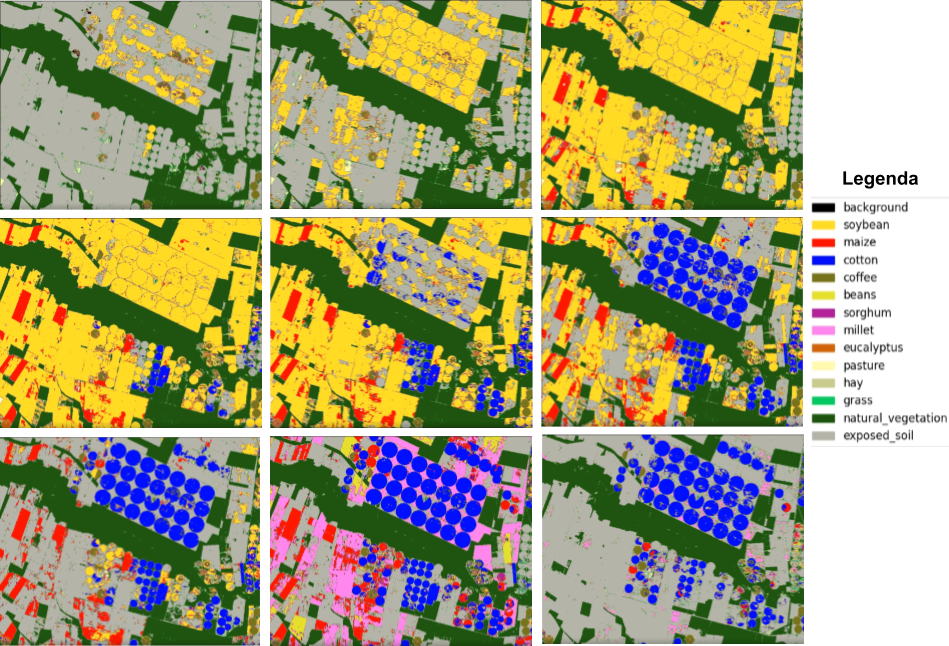
\includegraphics[width=0.8\textwidth]{figuras/serie_temporal_resultado.png}
\begin{tablenotes}
\item Vídeo completo disponível em: \url{https://www.youtube.com/watch?v=R6SwGzosLfM}.
\end{tablenotes}
\end{figure}

Na Figura \ref{fig:serie_temporal_resultado}, é possível observarmos o momento em que os talhões ainda estão com solo exposto, em seguida os talhões de soja e milho são plantados, permanecem por algum tempo em campo, e logo depois são colhidos, dando lugar à talhões de algodão e milhete, que também são colhidos e voltam a ficar com o solo exposto. 


\renewcommand{\cleardoublepage}{}
\renewcommand{\clearpage}{}
\vspace{5mm}
\chapter{Conclusão}

Neste trabalho, desenvolvemos uma metodologia que permite a geração de mapas do uso e cobertura da terra para a mesorregião do Extremo Oeste Baiano, no estado da Bahia, com uma periodicidade de 16 dias. A abordagem desenvolvida foi capaz de mapear treze classes de uso e cobertura da terra dentro da área de estudo, ao mesmo tempo em que permite acompanhar, a cada dezesseis dias, as mudanças que possam vir a ocorrer entre essas classes, como por exemplo, a mudança da classe 'exposed\_soil' para 'soybean' indicando o momento do plantio da soja e a mudança da classe 'soybean' para 'exposed\_soil' indicando o momento da colheita da soja. Aplicamos diversas técnicas para a compatibilização e correção das imagens de satélite, o que nós possibilitou trabalhar com imagens Landsat 8 e Sentinel 2A e 2B como se fossem uma única coleção de imagens de satélite. Treinamos três diferentes modelos de aprendizado de máquina, dois baseados no algoritmo \textit{Random Forest} e um baseado em redes neurais recorrentes utilizando a arquitetura de redes neurais \textit{Long short-term memory - LSTM}. O modelo baseado em LSTM foi o que apresentou os melhores resultados, com um \textit{F1-Score} médio de 79\% nas quatorze classes mapeadas (treze classes de uso e cobertura mais a classe de plano de fundo). O método apresentado aqui pode ser usado para mapear grandes áreas de uma forma relativamente rápida e a um custo relativamente baixo, comparado à interpretação manual de imagens de satélite feita por especialista. Para isso, o modelo baseado em LSTM, que apresentou os melhores resultados, precisaria ser retreinado com mais amostras coletadas na região de interesse para permitir que o modelo entenda toda a variabilidade das classes na nova região.

\renewcommand{\cleardoublepage}{}
\renewcommand{\clearpage}{}
\vspace{5mm}
\chapter{Links}

Disponibilizamos todos os dados utilizados para o treinamento e validação dos modelos, scripts desenvolvidos e vídeo explicativo através do repositório do projeto na plataforma GitHub: \url{https://github.com/saraivaufc/TCC-Inteligencia-Artificial}. 

\newpage

\referencias{elementos-pos-textuais/Bibliografia}


\end{document}

